\documentclass[final]{fhnwreport}       %[mode] = draft or final
                                        %{class} = fhnwreport, article, 
                                        %          report, book, beamer, standalone
\input{header}			                %loads all packages, definitions and settings
\addbibresource{literature/bibliography.bib}							
\title{Fachbericht}  		        %Project Title
\author{Anklin, Bobst, Horath}      				    %Document Type => Technical Report, ...
\date{\today}          				   %Place and Date

\begin{document}

%%---TITLEPAGE---------------------------------------------------------------------------------
\thispagestyle{empty}
%	\ohead{\includegraphics[scale=0.5]{Bilder/Logo_FHNW.jpg}}
	\begin{figure}
		 \vspace*{-\topskip}\vspace*{-\headsep}
		\includegraphics[scale=1]{graphics/fhnw_ht_logo_de.pdf}
	\end{figure}
	\begin{center}
		\vspace*{2cm}
		{\huge{\textbf{\thetitle}}}\\
		\vspace*{1cm}
		
		{\huge{Testumgebung und Performancevergleich von Zigbee, Thread und Bluetooth Mesh Netzwerken}}\\
		\vspace*{0.5cm}
		
		{\scshape\Large Bachelor Thesis - \theauthor \\} \Large{\today}
		\vfill
		
		
		\begin{normalsize}
			{\begin{tabbing}
						
					\textbf{Fachcoach:} \hspace{6cm}\= Matthias Meier\\
					\>Manuel Di Cerbo\\
					
					\\[0.4cm]
					
					\textbf{Team:} \>Raffael Anklin \\ \>Robin Bobst \\ \>Cyrill Horath
					\\[0.8cm]
					\textbf{Studiengang:} \>Elektro- und Informationstechnik
					\\[0.8cm]	\textbf{Semester:} \>Frühlingssemester 2020
			\end{tabbing}}
		\end{normalsize}
		\vfill
	\end{center}
\clearpage

%%---ABSTRACT----------------------------------------------------------------------------
\selectlanguage{english}				%ngerman or english
\thispagestyle{empty}
%\begin{abstract}
%This semester’s assignment was to design and implement a control-unit for a commercial 3D-Printer. The requirements, apart from proper functioning were that the printer should be able to operate independently from a PC, have wireless connectivity and be able to read and print from G-Code files. Although not explicitly required, further enhancements were highly encouraged. The approach adopted was to reverse-engineer available open-source solutions adding enhancements along the process. Due to prior experience of the team with it, the ATmega2560 was the chosen microcontroller for this project. All the circuit elements were integrated in a single PCB, including an ESP8266 wireless module to provide the printer with WLAN connectivity. The 24 V power supply circuit and all the connectors were designed to be compatible with a Creality3D Ender-3 Pro 3D printer model. The freeware Marlin was the most suitable software due to its compatibility with a broad range of hardware components. Marlin’s code has been modified to provided additional features and a customized visual identity to the printer. With additional sensors the control-unit provides the 3D-printer filament runout detection, filament blockage detection and sensorless homing. After manufacturing the PCB and flashing Marlin into the microcontroller a battery of tests validated the functionality of the control-unit. However, the filament blockage detection function could not have its sensitivity adjusted to a satisfactory degree and should, therefore, not be used. The end-product is a fully functional and enhanced control-unit for an Ender-3 Pro printer, which can be made available to students of this school as a support tool for their projects. 
%\end{abstract}	

\begin{abstract}
	Among the most popular low power mesh network protocols in free GHz ISM band the three mesh stacks Bluetooth Mesh, ZigBee and Thread are currently competing against each other. The assignment of this bachelor thesis was to build a consistent test framework for all three mesh-networks to benchmark them under realistic conditions. Due to better combability, the nRF52840 SoC from Nordic Semiconductors was the chosen microcontroller for all three network stacks. The benchmark is structured in two parts, a battery powered slave node and a master which is directly connected to a computer. The master node is responsible for controlling the measurement, whereas the slave nodes send benchmark messages to each other. These benchmark messages collect the necessary information to determine latency, RSSI, throughput and active radio time. For a better comparability an apartment house, an apartment and a labor environment were selected as different test benches. The Thread stack results the best in the different test benches. Because of its automatic routing it is able to adapt himself to the environment, as a result the latency of this stack is in every three benches similarly low. Bluetooth Mesh was able to reach the lowest latency with small payload. The ZigBee network stands out with its constant and low latency within one test bench. As a conclusion all of the three networks perform well in case of a home automation. Due to of their own assets and drawbacks it cannot be said this is the best mesh-stack. It depends on the application which mesh network performs the best.
\end{abstract}

\todo[inline]{Abstract durchlesen}


%%---TABLE OF CONTENTS-------------------------------------------------------------------
\pagenumbering{Roman}		
\selectlanguage{ngerman}				%ngerman or english
\tableofcontents
\clearpage

%%---TEXT--------------------------------------------------------------------------------
\pagenumbering{arabic}

%%Part 0 Allgemeiner Teil

\vspace*{4cm}
\begin{center}
\part{Benchmark-Konzept und Testumgebung}\label{BenchmarkKonzeptundTestumgebung}
\end{center}
\vspace*{\fill}
\clearpage

\section{Einleitung}\label{sec:Einleitung}

\todo[inline]{Allgemeine Einleitung in das Thema und die Arbeit. Die Gliederung des Berichts und die Aufteilung in Total 5 Teile soll erläutert werden --> Leseführung.}
\pagebreak

\clearpage

\section{Übersicht}\label{sec:Uebersicht}



\subsection{Ausgangslage und Aufgabenstellung}\label{subsec:AusgangslageundAufgabenstellung}
\todo[inline]{Die Aufgabenstellung soll kurz zusammengefasst werden (komplette Aufgabenstellung im Anhang) und die Ausgangslage abgegrenzt werden.}

\subsection{Vorarbeiten P5}\label{subsec:VorarbeitenP5}
\todo[inline]{Zusammenfassung über die Ergebnisse des P5. Ausserdem Erläuterung "Themenwechsel" zu Thesis (BL Mesh --> 3 Protokolle).}


\subsection{Ziel der Arbeit}\label{subsec:ZielderArbeit}
\todo[inline]{Zusammenfassung der Ziele aus Pflichtenheft (komplettes Pflichtenheft im Anhang). Validierung dieser Ziele erfolgt im Schlussteil dieses Berichts.}








\pagebreak

\vspace*{4cm}
\begin{center}
\part{Mesh Benchmark - Konzept und Umsetzung}\label{MeshBenchmarkKonzeptundTestumgebung}
\end{center}
\vspace*{\fill}
\clearpage

\section{Benchmark Konzept}\label{sec:BenchmarkKonzeptMeshNetzwerke}
Um die Performance der drei Mesh Stacks zu vergleichen wurde ein einheitliches Benchmark Konzept erarbeitet. Dieses definiert die Mesh Parameter, Testumgebungen, den Ablauf sowie sämtliche Messgrössen und Messreihen. Nachfolgend wird detailliert auf dieses Konzept eingegangen.

\subsection{Konzeptschema}\label{subsec:KonzeptschemaMesh}

Für den Vergleich der 3 Mesh Netzwerkstacks Bluetooth Mesh (BT Mesh), Thread und Zigbee wird ein vom Mesh Protokoll unabhängiges Testkonzept umgesetzt welches in der Abbildung \ref{fig:MeshTestKonzept} als Konzeptschema dargestellt ist.
Die Benchmark Slave Nodes (BSN) in der Abbildung als Sensoren und Aktoren mit unterschiedlichen Funktionalitäten dargestellt, bilden zusammen mit dem Benchmark Master Node (BMN) das zu testende Mesh Netzwerk.
Innerhalb des Netzwerks wird dessen Organisation vom jeweiligen Protokoll sichergestellt.
Das Testnetzwerk soll ein realitätsnahes Netzwerk nachbilden.
Eine Heimautomation in einem Einfamilienhaus oder Wohnung wird als Referenz angenommen in welchem jeweils nur gewisse Nodes untereinander Applikationsdaten austauschen.
Lichtschalter kommunizieren nur mit Lichtquellen und umgekehrt, sie tauschen jedoch keine Daten mit Temperatursensoren aus.
Diese unterschiedlichen Beziehungen innerhalb des Mesh Netzwerks sind in der Abbildung \ref{fig:MeshTestKonzept} angedeutet.

\begin{figure}[h]
	\centering
	\includegraphics[width=0.6\textwidth]{Mesh_Testkonzeptschema.png}
	\caption{Konzeptschema für den Ablauf eines Mesh Benchmarks.}\label{fig:MeshTestKonzept}
\end{figure}

Die Benchmark Management Station (BMS) welche mit dem BMN via USB/UART kommuniziert, ist zuständig für die Verwaltung und Verarbeitung des Benchmarks. Während eines Benchmark Prozesses sollen sämtliche Messungen jedoch unabhängig von der BMS durchgeführt werden damit allfällige Latenzzeiten der USB/UART Verbindung die Resultate nicht verfälschen.

\subsubsection{Messages}\label{subsubsec:Messages}
In der Abbildung \ref{fig:MeshTestKonzept} sind verschiedene Messages dargestellt. Dabei handelt es sich um die Nachrichten die zwischen den einzelnen Teilen des Testaufbaus versendet werden und schliesslich einen Benchmark ausmachen. Die Messages besitzen Funktionen:

\paragraph{Mesh Benchmark Message (MBM)}
Die MBM ist jene Message welche die eigentlichen Messdaten produziert und diese sogleich unter den BSN (Mesh Knoten) überträgt. Anhand dieser Messages werden die Parameter für den Vergleich der Protokolle gemäss Abschnitt \ref{subsec:VergleichswerteundMessgrössenMesh} erfasst. Bei den MBM handelt es sich also um eine Sammlung von Messages welche je nach gewünschtem Messwert in Form und Anzahl unterschiedlich ausfallen können.

\paragraph{Mesh Control Message (MCM)}
Die MCM beinhaltet die Parameter für die Benchmarks welche vom BMN an alle BSN übertragen werden. Ausserdem werden damit Kontrollbefehle für die Benchmarks wie beispielsweise \textit{Start/Stop} sowie \textit{Laufzeit, Wiederholrate usw.} übertragen.

\paragraph{Mesh Report Message (MRM)}
Die MRM ist jene Message welche die Messwerte von den BSN an den BMN übertragen. Gleichzeitig wird damit auch gleich signalisiert, dass die Messung abgeschlossen wurde und mögliche Fehler oder sonstige Status übermittelt.

\paragraph{Benchmark Control Message (BCM)}
Die BCM beschreibt die Nachrichten welche zur Steuerung eines Benchmarks von der BMS her dienen. Dabei handelt es sich um Befehle wie beispielsweise \textit{Start/Stop}. Die BCM werden via serieller USB-UART Schnittstelle von der BMS zum BMN übertragen.

\paragraph{Benchmark Report Message (BRM)}
Die BRM beschreiben Nachrichten welche den Status oder die Ergebnisse eines Benchmarks aus dem Mesh zurück an die BMS melden. Sie werden vom BMN initiiert und gelangen über eine die selbe USB-UART Schnittstelle wie die BCM zum BMS. Die BRM wird erst nach Abschluss des Benchmarks initiiert. Zuvor werden die Messdaten auf dem BMN zwischen gespeichert.


\subsubsection{Nodes}\label{subsubsec:Nodes}
Wie bereits angedeutet und in Abbildung \ref{fig:MeshTestKonzept} gezeigt, kann im Mesh Benchmark zwischen den folgenden 3 Node Typen unterschieden werden.

\paragraph{Benchmark Master Node (BMN)}
Der Benchmark Master Node bildet den zentralen Zugriffspunkt zum Mesh Netzwerk für den Benchmark. Über ihn werden Control und Report Messages versendet und empfangen. Im Zigbee Mesh Protokoll fungiert er zugleich Coordinator.


\paragraph{Benchmark Client Node (BCN)}
Der Benchmark Client Node repräsentiert beispielsweise einen Schalter in einer Lichtsteuerung. Im Benchmark Kontext ist er jene Instanz die MBM versendet.

\paragraph{Benchmark Server Node (BSN)}
Das Pendant zum BCN stellt der BSN dar. Er steht beispielsweise für eine Lichtquelle. Im Benchmark Kontext empfängt er die MBM die vom BCN versendet werden.


%\subsection{Testszenarien}\label{subsec:TestszenarienMesh}

%Die Benchmarks der Mesh Protokolle sollen mit unterschiedlichen Bedingungen getestet werden wobei grundsätzlich eine reelle Anwendung nachgebaut werden soll. Zum einen gibt es unterschiedliche Beziehungen innerhalb des Mesh Netzwerks, zum anderen werden Testumgebungen unterschieden.

%\subsubsection{Mesh Beziehungen}\label{subsubsec:MeshBeziehungen}
%
%\todo[inline]{Raffi:  Ist diese Information Relevant für das verständniss des Benchmarks?}
%
%Innerhalb eines Mesh Netzwerks können 4 Beziehungen zwischen den Nodes für die Benchmarks unterschieden werden. Üblicherweise kommen mehrere oder sogar alle 4 Beziehungen innerhalb eines Netzwerkes gleichzeitig zum Einsatz. Abbildung \ref{fig:MeshTestBeziehungen} zeigt die Beziehungen.
%
%\begin{itemize}
% 	\item \textcolor{red}{Rot} stellt eine einfache P2P Verbindung ohne Hop dar. Beispielweise schaltet ein einzelner Schalter eine einzelne, definierte Lichtquelle
% 	\item \textcolor{orange}{Orange} ist eine many-to-one Verbindung in welcher mehrere Lichtschalter die selbe Lichtquelle schalten.
% 	\item \textcolor{cyan}{Blau} ist eine klassiche one-to-many Topologie dargestellt in welcher beispielsweise ein Schalter mehrere Lichtquellen bedient.
% 	 \item \textcolor{green}{Grün} dargestellt ist eine indirekte P2P Verbindung mit. Das bedeutet, dass Schalter und Lichtquelle keine direkte Verbindung zueinander haben und daher Mesh-typisch via einem oder mehreren Hops kommuniziert.
%\end{itemize}
%
%
%\begin{figure}[H]
%	\centering
%	\includegraphics[width=1.0\textwidth]{Mesh_Test_Beziehungen.png}
%	\caption{Beziehungen zwischen den Mesh Nodes innerhalb eines Benchmarks.}\label{fig:MeshTestBeziehungen}
%\end{figure}

\subsection{Testumgebungen und Messaufbau}\label{subsubsec:TestumgebungenundMessaufbau}

%\subsubsection{Testumgebungen und Messaufbau}\label{subsubsec:TestumgebungenundMessaufbau}

Unterschiedliche Testumgebungen sollen die Benchmarks und schlussendlich den Vergleich der 3 Mesh Protokolle aussagekräftiger machen.
Nachfolgende Umgebungen mit den entsprechenden Eigenschaften sollen getestet werden.
Die Abbildungen zu den Testumgebungen zeigen jeweils die Platzierung der Nodes sowie deren Funktion und Gruppen Zugehörigkeit. Die Farbe Grün identifiziert den Node als Client Node während Blau für einen Server Nodes steht. Die Nummerierung zeigt welcher Node zu welcher Adressgruppe gehört. Ein Client Node in Gruppe 1 sendet jeweils Nachrichten zu allen Server Nodes in der selben Gruppe.

\paragraph{Labor}
Der Laboraufbau ist ein Extremtest welcher die Leistungsgrenzen der Protokollstacks ausloten soll. Dabei werden die Nodes auf einem Raster gemäss Abbildung \ref{fig:AnordnungLaborTestumgebungMessumgebung1} angeordnet. Die genauen Abmessungen sind der Abbildung zu entnehmen.
\begin{itemize}
	\item Testaufbau unter Laborbedingungen auf engstem Raum.
	\item Ausgeglichene Anzahl Sensoren und Aktoren.
	\item Sehr Hohe Node-Dichte.
	\item Geringe bis keine Störbeeinflussung durch die Umgebung zu  erwarten.
	\item Die Mesh-Beziehungen werden künstlich bestimmt sodass einfache P2P Verbindungen mit oder ohne Hop entstehen.
\end{itemize}


\begin{figure}[H]
\centering
\includegraphics[width=0.7\textwidth]{Testaufbau_Labor.png}
\caption{Anordnung Labor Testumgebung, Messumgebung 1}\label{fig:AnordnungLaborTestumgebungMessumgebung1}
\end{figure}

\paragraph{Einfamilienhaus}
Die Testgeräte werden in einem Einfamilienhaus installiert und repräsentieren damit eine flächendeckende Heim-Automatisierung. Folgende Eingenschaften soll diese Messung abdecken:
\begin{itemize}
	\item Einfamilienhaus über mehrere Etagen.
	\item Node-Dichte relativ gering.
	\item Kleine Beeinflussung durch Nachbarsysteme sind zu erwarten.
	\item Sämtliche Mesh-Beziehungen gemäss \ref{subsubsec:MeshBeziehungen} kommen vor und werden durch die bestehende Infrastruktur bestimmt.
\end{itemize}

Die Abbildung \ref{fig:Messumgebung2Einfamilienhaus} zeigt die Platzierung der Nodes auf den 4 Etagen des Einfamilienhauses.

\begin{figure}[H]
	\centering
	\includegraphics[width=\textwidth]{Plan_Haus_Raffi.png}
	\caption{Platzierung der Nodes im Einfamilienhaus}\label{fig:Messumgebung2Einfamilienhaus}
\end{figure}
	
\paragraph{Wohnung}
Ebenfalls als Heim-Automatisierung gedacht werden die Messungen in einer Wohnung durchgeführt.
\begin{itemize}
	\item Wohnung über eine Etage in einem Mehrfamilienhaus
	\item Anzahl Sensoren und Aktoren vergleichbar gross.
	\item Node-Dichte höher als im Haus.
	\item Mögliche Störeinflüsse durch andere Systeme von Nachbarn sind zu erwarten.
	\item Sämtliche Mesh-Beziehungen gemäss \ref{subsubsec:MeshBeziehungen} kommen vor und werden durch die bestehende Infrastruktur bestimmt.
\end{itemize}

Bei der Wohnung handelt es sich um eine 3.5 Zimmer Wohnung mit einer Wohnfläche von 122 Quadratmetern. Die genauen Abmessungen sowie die Platzierung der Nodes ist in Abbildung \ref{fig:PlatzierungderNodesinMessumgebung3} zu sehen.

\begin{figure}[H]
	\centering
	\includegraphics[width=\textwidth]{Plan_Wohnung_Cyrill_Nodes_Placement.png}
	\caption{Platzierung der Nodes in Messumgebung 3 (Wohnung)}\label{fig:PlatzierungderNodesinMessumgebung3}
\end{figure}




\subsection{Ablauf}\label{subsec:AblaufMesh}

Ein Mesh Benchmark folgt einem klar definierten Ablauf. Die Abbildung \ref{fig:MeshTestKonzept} zeigt das Testkonzept in welchem auch der Ablauf eines Benchmarks bereits angedeutet ist.

\begin{enumerate}
	\item \textbf{Benchmark User-Init:}\\
	Im Config File auf dem BMS werden die gewünschten Parameter definiert, die Konfiguration verteilt und der Benchmark durch den Benutzer gestartet.
	\item \textbf{Benchmark Init BMN:}\\
	Die Parameter werden an den BMN übergeben welcher diese wiederum an alle teilnehmenden BSN weiterleitet. Mit einem Startsignal vom BMN wird der Benchmark auf den BSN gestartet.
	\item \textbf{Benchmark Prozess:}\\
	Die BSN führen den Benchmark Prozess mit den definierten Parametern aus. Dies geschieht autonom und jeweils nur zwischen den entsprechenden BSN die gemäss Benutzerkonfiguration in einer direkten Beziehung zueinander stehen (siehe Mesh Beziehungen \ref{subsubsec:MeshBeziehungen}). Die entstandenen Messdaten werden auf den BSN zwischengespeichert und nach Ablauf des Benchmarks ins Flash geschrieben.
	\item \textbf{Reporting:}\\
	Nach Ablauf der Benchmark Zeit werden die Messdaten an den BMN übertragen. Dies erfolgt gesteuert durch den BMN welcher die Daten bei einem BSN nach dem anderen abfragt und direkt an das BMS weiterleitet.
	\item \textbf{Finish:}\\
	Der BMN kontrolliert ob er die Daten von sämtlichen BSN korrekt auslesen konnte und bestätigt das Ende der Messung gegenüber dem BMS.
	\item \textbf{Auswertung:}\\
	Das BMS beendet den Benchmark Vorgang und speichert die Messdaten in seiner Datenbank ab. Von dort können die Daten gelesen und mit Excel ausgewertet werden.
\end{enumerate}

%\subsection{Anforderungen}\label{subsec:SoftwareAnforderungen}
%\todo[inline]{Titel ändern. Und Text an restliches Kapitel anpassen.}
%Wie bereits im Abschnitt \ref{sec:Abgrenzung} wurden die Anforderungen in der Aufgabenstellung (siehe Anhang \ref{app:Aufgabenstellung}) sowie im Pflichtenheft (siehe Anhang \ref{app:Pflichtenheft}) vorgängig festgelegt. Im Fokus steht das erfassen der wichtigsten Messgrössen welche nachfolgend aufgeführt werden.
%
%\begin{itemize}
%	\item \textbf{Latenzzeit}: Bestimmung der Latenzzeit in Millisekunden zwischen den Teilnehmern. Die Genauigkeit sollte bei $+/-$1 ms liegen.  
%	\item \textbf{Anzahl Hops}: Bestimmung der Anzahl Hops, über welche eine Nachricht übermittelt wird.
%	\item \textbf{Datenrate}: Messen der Datenrate in Bytes/s, welche zwischen zwei Teilnehmern erreicht wurde. 
%	\item \textbf{RSSI}: Erfassen des RSSI-Werts der eingehenden Pakete.
%	\item \textbf{Paketverlust}: Pakete zählen, welche ihr Ziel nicht erreicht haben.  
%	\item \textbf{Aktive Radio Zeit}: Erfassen der aktiven Radio-Zeit um den Energieverbrauch abschätzen zu können. 
%\end{itemize}
%
%
%Die Erfassung muss in allen Mesh-Netzwerken möglich sein. Um die Messresultate vergleichen zu können müssen die gleichen Ausgangslagen vorliegen, sowie die selben Messmethoden angewendet werden. 



\subsection{Vergleichswerte und Messgrössen}\label{subsec:VergleichswerteundMessgrössenMesh}
Beim Vergleich der Mesh Protokolle wird zwischen Vergleichswerten und Messgrössen unterschieden. Vergleichswerte sind meist aus einer oder mehreren Messgrössen berechnete Werte die einen aussagekräftigen Vergleich ermöglichen.

\subsubsection{Vergleichswerte}\label{subsubsec:Vergleichswerte}
Im Pflichtenheft zu dieser Arbeit (Anhang \ref{app:Pflichtenheft}) wurden die Testkriterien für den Vergleich bereits ausführlich behandelt.
Folgende Vergleichswerte kommen nun in der Auswertung effektiv zum Tragen:

\begin{itemize}
	\item \textbf{Latenzzeit}: Bestimmung der Latenzzeit in Millisekunden eines Pakets das über das Mesh vom Client zum Server versendet wird.  
	\item \textbf{Anzahl Hops}: Bestimmung der Anzahl Hops, über welche eine Nachricht übermittelt wird.
	\item \textbf{Datenrate}: Messen der Datenrate in Bytes/s, welche zwischen zwei Teilnehmern erreicht wurde. 
%	\item \textbf{RSSI}: Erfassen des RSSI-Werts der eingehenden Pakete.
	\item \textbf{Paketverlust}: Pakete welche ihr Ziel nicht erreichen konnten werden gezählt um so eine Paketverlustrate zu ermitteln.
	\item \textbf{Aktive Radio Zeit}: Zur Abschätzung des Energieverbrauchs der Nodes im Mesh Betrieb, wird die Aktivdauer der Radio Schnittstelle gemessen.
\end{itemize}


\subsubsection{Messgrössen}\label{subsubsec:Messgrössen}

Um diese Werte zu erfassen sind spezifische Messgrössen gefragt die auf den Nodes direkt erfasst werden können.
Die untenstehende Auflistung zeigt die auf den Mesh Nodes erfassten Messgrössen, deren Generierung und wie diese in der Auswertung verwendet werden.


\paragraph{Message Timestamp}
Zur Bestimmung der Latenzzeit eines Pakets das über das Mesh Netzwerk versendet wird, wird beim Senden sowie beim Empfangen ein Message Timestamp erfasst.
Die unter den Nodes synchronisierte Zeit gibt Aufschluss darüber wie lange das Paket unterwegs war. Die Berechnung der Latenzzeit wird jedoch erst bei der Analyse auf dem BMS durchgeführt.

\paragraph{Number of Hops}
Die oben erwähnte Latenzzeit ist in einem Mesh Netzwerk abhängig vom Weg den ein Paket bei der Übermittlung genommen hat. Mit jedem Hop nimmt die Latenzzeit zu.
Deshalb wird beim Server Node die Anzahl Hops die das Paket genommen hat aus dem Message Header ausgelesen und für die Bestimmung der Latenzzeit abgespeichert.

\paragraph{Source-, Destination-, Group-Address}
Aufgrund der veränderlichen Beziehungen von Client und Server Nodes ist die Zuordnung von Quell- und Zieladresse eines Pakets ebenfalls nicht statisch. Aus diesem Grund werden auf allen Nodes die Quell-, Ziel- und Gruppenadressen der Pakete ausgelesen. 
Somit kann das Benchmark Paket eindeutig identifiziert und in der Auswertung erfasst werden.
Die Adressinformationen werden aus dem Message Header des Mesh Pakets ausgelesen oder im Falle des Client Nodes mit der Benchmark Control Message übermittelt.

\paragraph{Message ID}
Als Payload im Mesh Paket versendet, identifiziert die Message ID das Paket zusammen mit den Adressinformationen eindeutig. So kann Paketverlust wie auch die Latenzzeit erfasst werden.

\paragraph{RSSI}
Der RSSI (Received Signal Strength Indication) wird auf dem Server Node auf MAC Ebene erfasst und zeigt die Empfangsqualität der Übertragung. Dies kann bei der Analyse des Benchmarks als weiterer Indikator für Paketverlust und Latenzzeit verwendet werden.

\paragraph{Aktive Radio Zeit}
Die Zeit in der die Radio Schnittstelle aktiv ist wird auf dem Node direkt gestoppt und gespeichert.


\subsection{Messreihe}\label{subsec:Messreihe}
Um die Mesh Protokolle einem möglichst fairen Vergleich zu unterziehen, werden pro Testumgebung eine Reihe an Messungen durchgeführt. Die Tabelle \ref{tab:ParameterBenchmarkMessreihe} zeigt Total 8 Messreihen mit den entsprechenden Parametern.

\begin{table}[h]
\centering
\begin{adjustbox}{width=1\textwidth}
\begin{tabular}{|c|c|c|c|c|c|c|c|c|} 
\cline{2-9}
\multicolumn{1}{c|}{} & \multicolumn{5}{c|}{Benchmark Parameter} & \multicolumn{3}{c|}{Messaufbau} \\ 
\hline
\textbf{\#}  & \textbf{Msg. Gen.}  & \textbf{Duration} & \textbf{Msg. Cnt.}  & \textbf{Payload }  & \textbf{Disturbance}  & \textbf{Labor}  & \textbf{Haus}  & \textbf{Wohnung}  \\ 
\hline
1 & Rand & 600s & 60 & Small & No & x & x & x \\ 
\hline
2 & Seq & 600s & 60 & Small & No & x & x & x \\ 
\hline
3 & Rand & 600s & 60 & Large & No & x & x & x \\ 
\hline
4 & Seq & 600s & 60 & Large & No & x & x & x \\ 
\hline
5 & Rand & 600s & 600 & Small & No & x & x & x \\ 
\hline
\multicolumn{1}{c}{} & \multicolumn{1}{c}{} & \multicolumn{1}{c}{} & \multicolumn{1}{c}{} & \multicolumn{1}{c}{} & \multicolumn{1}{c}{} & \multicolumn{1}{c}{} & \multicolumn{1}{c}{} & \multicolumn{1}{c}{} \\ 
\hline
6 & Rand & 600s & 60 & Small & Yes & x &  &  \\ 
\hline
7 & Seq & 750s & 10 & Small & No & x &  &  \\ 
\hline
8 & Seq & 750s & 10 & Large & No & x &  &  \\
\hline
\end{tabular}
\end{adjustbox}
\caption{Parameter Benchmark Messreihe}
\label{tab:ParameterBenchmarkMessreihe}
\end{table}

Die Erläuterungen über die Bedeutung der Parameter ist in der folgenden Übersicht \ref{tab:BedeutungBenchmarkParameter} zu finden. 

\begin{table}[h]
\centering
\begin{adjustbox}{width=1\textwidth}
\begin{tabular}{lll} 
\toprule
Parameter: & Gültige Werte: & Bedeutung: \\ 
\hline
Msg. Gen & Seq/Rand & Nachrichten Generierung Sequentiell oder Pseudozufällig \ref{subsec:TrafficGeneration}. \\
Duration & Ganze Zahlen & Dauer eines Benchmarks angegeben in Sekunden. \\
Msg. Count & Ganze Zahlen & Anzahl der Nachrichten die pro Client Node versendet werden.\\
Payload & Small/Large & Grosse oder Kleine Payload gemäss Definition in Tabelle.\\
Disturbance & Yes/No & \begin{tabular}[t]{@{}l@{}}Gewollte Störung durch P2P Testinfrastruktur auf\\dem selben Channel. \end{tabular} \\
\bottomrule
\end{tabular}
\end{adjustbox}
\caption{Bedeutung Benchmark Parameter}
\label{tab:BedeutungBenchmarkParameter}
\end{table}

Die Messungen 1 bis 5 werden in allen drei Messaufbauten durchgeführt. So werden die Unterschiede der Topologien ersichtlich.
Die Messungen 6 bis 8 hingegen werden nur im Laboraufbau durchgeführt damit allfällige Externe Störeinflüsse ausgeschlossen werden können und das Mesh Netzwerk unter Extrembedingungen getestet werden kann.

Bei der Messung mit dem Index 6 handelt es sich um ein Benchmark welcher mit der P2P Testinfrastruktur gestört wird. So soll die Störimmunität des Mesh Stacks getestet werden.
Die Messungen 7 und 8 wurden aufgrund der Erfahrungen die mit den Resultaten der Messungen 1 bis 6 gesammelt werden konnten, nachträglich ergänzt. In Abschnitt \ref{sec:Validierung} wird genauer auf diese Problematik eingegangen.
Die Dichte der Nachrichten ist bei diesen Messungen deutlich tiefer.





\subsection{Allgemeine Benchmark Parameter}\label{subsec:AllgemeineBenchmarkParameter}

Die oben erwähnten Messreihen haben nebst den variablen Parametern einige allgemeingültige Benchmark Parameter die in der Tabelle \ref{tab:AllgemeineBenchmarkParameter} aufgeführt sind.
Diese sind für sämtliche Messungen innerhalb des jeweiligen Mesh Protokolls gültig.
Die ersten vier Parameter \textit{Group addressing mode, Application Layer, MAC Layer} sowie \textit{Mesh Node Type} sind protokollabhängig und deshalb bei allen drei Mesh Stacks unterschiedlich.
Da sich diese Parameter innerhalb des jeweiligen Protokolls unterschiedlich umsetzen lassen sind die gewählten Werte resp. Funktionen hier aufgelistet.
Deren Funktionsweise wird in separaten Abschnitten noch detailliert behandelt.

Beim \textit{Group addressing mode} wird zwischen Broadcast bei BT Mesh, Multicast bei Thread und Unicast bei Zigbee unterschieden. Gemäss Definition im Pflichtenheft soll jeweils eine Gruppenadressierung stattfinden. Zigbee bietet zwar eine solche Möglichkeit eines Multicasts jedoch wird dieser schliesslich als Broadcast umgesetzt was eine deutliche Limitierung der Performance verursacht.
Aufgrund dieser Erfahrung und der Erkenntnis dass marktübliche Lichtsteuerungen\footnote{Analyse mittels Sniffer Trace einer IKEA Tradfri Lichtsteuerung.} nur selten ein solches Multicast Prinzip verwenden, wird die Adressierung im Benchmark gerichtet (Unicast) vorgenommen (siehe auch Abschnitt \ref{subsubsec:Adressierung}).
Das bedeutet die Nachrichten werden nicht an eine Gruppenadresse sondern direkt an die jeweilige Node Adresse gesendet. Bei mehreren Servern innerhalb einer Gruppe werden also auch mehrere Nachrichten versendet.



\begin{table}[h]
\centering
\begin{tabular}{lccc} 
\toprule
 & BT Mesh & Thread & Zigbee \\ 
\hline
Group addressing mode & Broadcast & Multicast & Unicast \\
Application Layer & Models & CoAP [\ref{subsec:CoAP}] & ZCL [\ref{subsubsec:ApplicationLayer}] \\
MAC-Layer & BLE 1 Mbit & IEEE 802.15.4 & IEEE 802.15.4 \\
Mesh Node Type & Relay & FTD [\ref{par:FullThreadDevice}] & Zigbee-Router [\ref{subsec:NetzaufbauundTopologie}] \\
Mesh Node Cnt. & 50 & 50 & 50 \\
Client/Server Verhältnis & 25/25 & 25/25 & 25/25 \\
Message Ack (Appl. Layer) & No & No & No \\
Payload Size Small (Byte) & 8 & 8 & 8 \\
Payload Size Large (Byte) & 32 & 50 & 50 \\
\bottomrule
\end{tabular}
\caption{Allgemeine Benchmark Parameter}
\label{tab:AllgemeineBenchmarkParameter}
\end{table}

In den Punkten \textit{Mesh Node Cnt., Client/Server Verhältnis, Message Ack}, sowie \textit{Payload Size Small} unterscheiden sich die Benchmarks der drei Protokolle nicht.
Sämtliche Benchmarks werden mit 50 Mesh Nodes durchgeführt. Davon sind jeweils gleich viele Client Nodes wie Server Nodes \ref{subsubsec:Nodes}.
Die Benchmark Nachrichten werden auf dem Application Layer \textit{unacknowledged} versendet. Wenn also ein Paket sein Ziel nicht erreicht, wird dies vom Sender nicht registriert und das Paket nicht erneut übertragen.

Die \textit{Payload Size Small} mit der Grösse von 8 Byte soll eine kleine Nachricht repräsentieren wie sie beispielsweise beim Dimmen einer Lampe versendet wird.
Mit der \textit{Payload Size Large} hingegen soll eine vergleichsweise grosse Payload simuliert werden die über das Mesh übertragen wird.
Die beiden Protokollstacks Thread und Zigbee erlauben dank IEEE 802.15.4  eine totale Framegrösse von 127 Byte.
Abzüglich der Grösse der Header bieten die Protokolle noch Platz für eine Payload von ca. 50 Byte. Je nach Implementation der Protokolle variiert die Header Grösse und die Payload kann entsprechend erhöht werden.
BT Mesh hingegen beginnt bereits bei einer Payload Grösse von 8 Byte mit der Fragmentierung. Somit werden bei den 32 Byte für die \textit{Payload Size Large} bereits 4 Frames versendet. Diverse Tests haben ergeben, dass hier der BT Mesh Stack an seine Leistungsgrenze stösst.
Aus diesem Grund wäre eine weitere Erhöhung der Payload nicht sinnvoll.



\subsection{Traffic Generation}\label{subsec:TrafficGeneration}

Die in Tabelle \ref{tab:BedeutungBenchmarkParameter} erwähnte Message Generation ist im Benchmark verantwortlich für die Verteilung der Benchmark Nachrichten über die Nodes in Abhängigkeit der Zeit. So wird bestimmt wie der Traffic innerhalb des Netzes sowie auf den einzelnen Nodes generiert wird.
Dabei werden die folgenden zwei Modi unterschieden:

\paragraph{Random}\label{par:Random}
Im Modus \textit{Random} werden die Zeitpunkte für den Versand einer Nachricht sogenannt pseudozufällig generiert. Dies bedeutet, dass jedem Client Node eine Liste von einmalig zufällig generierten Werten zugewiesen wird.
Aus dieser Liste werden nur so viele Werte gelesen wie es Nachrichten zu versenden gilt. Diese werden schliesslich nach Grösse sortiert und über den gesamten Benchmark Zeitraum gelegt woraus nun die Zeitpunkte für den Versand der Nachrichten entstehen.
Ein solche Methode erlaubt es die Zeitpunkte reproduzierbar zu machen und identisch auf alle 3 Mesh Stacks anzuwenden.

\paragraph{Sequentiell}\label{par:Sequentiell}
Mit der \textit{Random} Methode kann die Belastung eines Nodes sowie des gesamten Netzes zwischenzeitlich stark ansteigen.
Um dies zu verhindern, kann der Traffic Generation Modus \textit{Sequentiell} gewählt werden.
Dabei werden die Nachrichten in regelmässigen Zeitschlitzen gemäss \ref{eq:TrafficGenerationSeq} pro Node versendet. Die Reihenfolge der Nodes bleibt jeweils die selbe.


\begin{equation}\label{eq:TrafficGenerationSeq}
T_{Msg\_send} =  \frac{T_{Bench\_Duration}}{(Msg\_Cnt \cdot 25)} \cdot NodeID \cdot i_{Msg}
\end{equation}

\begin{small}
\begin{center}
\begin{tabular}{ll}
$T_{Msg\_send}$ & Zeitpunkt zu welchem die Nachricht gesendet wird.\\
$T_{Bench\_Duration}$ & Benchmark Dauer (siehe \ref{tab:ParameterBenchmarkMessreihe})\\
$Msg\_Cnt$ & Anzahl Nachrichten die versendet werden.\\
$NodeID$ &Identifikationsnummer des Nodes. \\
$i_{Msg}$ & Message Index
\end{tabular}
\end{center}
\end{small}





\subsection{Messdatenerfassung und Auswertung}\label{subsec:MessdatenerfassungundAuswertung}

Für die Messdatenerfassung und Auswertung wird keine dedizierte Hardware verwendet. Die eigentlichen Messwerte die in Abschnitt \ref{subsec:VergleichswerteundMessgrössenMesh} erläutert sind, werden auf den Mesh Nodes direkt erfasst und erst im RAM und später im Flash des Microcontrollers zwischen gespeichert. Von dort werden sie mittels BRM (Benchmark Report Message) an den BMN übertragen.
Auf den Mesh Nodes inkl. BMN findet noch keine Auswertung der Daten statt.
Diese wird an das BMS ausgelagert.
Das BMS empfängt die BRM via CLI (Command Line Interface) und speichert die Messwerte in einem Excel CSV File ab. Dazu kommt ein Python Skript zum Einsatz (siehe \ref{subsubsec:Benchmark}).
Mittels einem weiteren Python Skript und manueller Bearbeitung in Excel können die so erfassten Daten ausgewertet werden.


\subsubsection{Identifizierung Benchmark Slave Node}\label{subsubsec:NodeIdentification}

Die verschiedenen Benchmark Slave Nodes (BSN) werden mithilfe ihrer MAC-Adresse identifiziert.
Jedem nRF52840 SoC wird eine 48-bit lange Adresse während der Produktion eingebrannt. Dabei handelt es sich um zufällig generierte Werte.
Zur Identifizierung im Benchmark werden nur die letzten 32-bit dieser MAC-Adresse verwendet.
Auf dem nRF-52840-Dongle ist die Adresse auf der Rückseite angegeben (siehe Abbildung \ref{fig:MACAdresseDongle}) und kann so einfach abgelesen werden.

\begin{figure}[H]
	\centering
	\includegraphics[width=0.3\textwidth]{Donge_MAC_Address.jpg}
	\caption{MAC Adresse nRF52840-Dongle}\label{fig:MACAdresseDongle}
\end{figure}


\subsubsection{Konfiguration Benchmark Slave Node}\label{subsubsec:NodeConfiguration}
Zur Konfiguration der BSN dient ein Excel-File. Darin sind alle Nodes mit ihren Konfigurations-Parametern aufgelistet. Die folgenden Angaben sind in einem Konfigurations-Eintrag enthalten. 

\begin{itemize}
	\item \textit{\textbf{Nummer:}} Gibt die Nummer des zu konfigurierenden Teilnehmers an.
	\item \textit{\textbf{Firmware:}} Verweis auf das Firmware-File mit welchem der Teilnehmer geflasht wird.
	\item \textit{\textbf{Dev ID:}} Gibt die letzten 32bit der MAC-Adresse des zu konfigurierenden Teilnehmers an (siehe Abschnitt \ref{subsubsec:NodeIdentification})
	\item \textit{\textbf{Group ID:}} Index der Gruppe zu der der Teilnehmer gehört. (siehe Abschnitt \ref{subsubsec:TestumgebungenundMessaufbau})
	\item \textit{\textbf{Node ID:}} Die Node ID wird nur bei Clients benötigt. Dieses Feld gibt an welche pseudozufälligen Werte im Traffic Generation Modus Random (siehe Abschnitt \ref{subsec:TrafficGeneration}) benutzt werden.
	\item \textit{\textbf{Ack:}} Einschalten des Sendens von Acknowledged Messages.
	\item \textit{\textbf{Add Payload Len:}} Gibt die Anzahl Bytes an, welche zusätzlich zu jeder Nachricht angehängt werden um die Gesamtgrösse des Pakets zu verändern.
	\item \textit{\textbf{Traffic Gen Mode:}} Gibt die Art an wie der Traffic generiert wird (siehe Abschnitt \ref{subsec:TrafficGeneration}).  
	\item \textit{\textbf{DST\_Node\_1-3:}} Gibt die Nummer des Servers an, welcher im Unicast Addressing Mode als Ziel verwendet wird. Es können Total drei Einträge definiert werden.  
	\item \textit{\textbf{DST\_MAC\_1-3:}} Gibt die MAC-Adresse des Servers an, welcher im Unicast Addressing Mode als Ziel verwendet wird. Diese Felder sind von den Feldern \textit{DST\_Node\_1-3} abhängig. 
\end{itemize}

Mithilfe eines CLI Befehls können die einzelnen Teilnehmer konfiguriert werden (siehe Abschnitt \ref{subsubsec:CLI}). Mithilfe des Python Scripts aus Abschnitt \ref{subsubsec:Configurator}, wurde dieser Vorgang automatisiert. 

\subsubsection{Starten einer Messung}\label{subsubsec:StartofMeassurment}
Beim Starten einer Messung über das CLI müssen die folgenden Parameter dem Startbefehl mitgegeben werden: 

\begin{itemize}
	\item \textit{\textbf{BenchmarkTime}} Die Zeit wie Lange der Benchmark dauert in Sekunden. 
	\item \textit{\textbf{BenchmarkMsgCnt}} Die Anzahl Nachrichten, welche pro Client versendet werden sollen. 
\end{itemize}

Die Eingabe des Befehls erfolgt gemäss Abschnitt \ref{subsubsec:CLI}. 


\subsubsection{Einholen der Messdaten}\label{subsec:GetNodeReports}

Mithilfe eines CLI-Befehls aus Abschnitt \ref{subsubsec:CLI} können die Messdaten eingeholt werden. Durch das Python Script aus Abschnitt \ref{subsubsec:BenchmarkandReporter}, wurde dieser Vorgang automatisiert. 


\subsection{Messerwartung}\label{subsec:Messerwartung}
Wie in der Übersicht \ref{subsec:VorarbeitenP5} bereits erwähnt, konnte im Rahmen der Vorarbeiten zu dieser Thesis der BT Mesh Stack bereits vertieft untersucht und erste Erfahrungen damit gesammelt werden. Bei den beiden anderen Stacks, Thread und Zigbee musste dies erst noch erfolgen.
Bei eben diesen Vorarbeiten konnten bereits deutliche Unterschiede zwischen den Stacks beobachtet werden, hauptsächlich verursacht durch das Routing bei Thread und Zigbee sowieso das Flooding-Mesh Prinzip bei BT Mesh.
Aufgrund dieser Erfahrungen wird erwartet, dass die beiden auf dem IEEE 802.15.4 Standard aufbauenden Protokolle klare Vorteile haben werden da die Nachrichtenzustellung durch das Routing effizienter realisiert werden kann.
Hingegen könnte BT Mesh Vorteile haben bei kleiner Belastung des Netzes.


\pagebreak

\clearpage
\section{Point to Point Testinfrastruktur}\label{sec:PointtoPointTestinfrastruktur}

Im Nachfolgenden Abschnitt wird auf die Point to Point (P2P) Messung eingegangen. Ziel ist es die Verbindung auf MAC-Layer auszumessen und die aus Abschnitt ... aufgelisteten Messdaten zu erfassen. Dazu wird im folgenden auf das Messkonzept, den Messablauf und technische Einzelheiten eingegangen. 

\subsection{Konzept}\label{sec:KonzeptP2P}

Zur Realisierung der Point to Point Testinfrastruktur wurde auf eine \textit{One to Many} (1:n) Messprinzip gesetzt (auch als Broadcasting bekannt). Dies hat den Vorteil das mehrere Verbindungen gleichzeitig ausgemessen werden können. Der Nachteil dabei ist, dass die Messpfade nur unidirektional charakterisiert werden (nur von Master zu Slave oder Uplink-Pfad). Die Abweichung zwischen Up- und Downlink Pfad können durch wiederholen der Messung mit vertauschten Standorten verifiziert werden. 

\begin{figure} [H]
	\centering
	\includegraphics[width=0.8\textwidth]{Konzeptschema_P2P.png}
	\caption{Konzeptschema P2P Testinfrastruktur}
	\label{fig:KonzeptschemaP2P}
\end{figure}

Das in Abbildung \ref{fig:KonzeptschemaP2P} gezeigte Konzept besteht aus einer Managment Station, einem Master- und mehreren Slave Nodes. Über die Management Station können Messresultate angezeigt, sowie Messparameter eingestellt werden. Als Ausgangspunkt zur Messung dient der MN (Master Node). Er koordiniert den Messablauf und sendet \textit{Probe Packets} an alle SN (Slave Nodes). Diese Protokollieren die Anzahl empfangener \textit{Probe Packets} und melden ihre Messresultate an den MN zurück. Nach Empfang aller Resultate leitet der MN alle Messergebnisse an die MS weiter. Dort werden dem Benutzer die Messdaten dargestellt. Details zum Ablauf sind in Abschnitt \ref{sec:SoftundFirmware} aufgeführt. Eine mögliche Anwendung der Testinfrastruktur wird im folgenden Abschnitt \ref{sec:TestszenarienP2P} beschrieben.  

\subsection{Testszenarien}\label{sec:TestszenarienP2P}

Die P2P Testinfrastruktur ist als einfach zu bedienendes Tool konzipiert. Es kann eingesetzt werden um den Aufbau von PAN-Netzwerken zu optimieren. Mithilfe des Tools können zu Beispiel die Standorte der Teilnehmer eines Zigbee, Thread oder Bluetooth Mesh Netzwerks optimal gewählt werden. Zudem lassen sich während eines Messvorgangs gezielt Störungen in ein solches Netzwerk einbringen. Dadurch können die Netzwerke auf Störsicherheit geprüft werden. 

\todo[inline]{Testumgebungen sowie die Beziehungen der Knoten innerhalb der Point to Point Messung beschreiben.}

\subsection{Ablauf}\label{sec:AblaufP2P}
\todo[inline]{Ablauf eines Point to Point MAC Layer Benchmarks aus Anwendersicht beschreiben.}

\subsection{Messgrössen}\label{sec:MessgrössenP2P}
\todo[inline]{Erläuterung der Messgrössen die erfasst werden sollen. Inkl. Beschreibung wie dies technisch umgesetzt wird.}

\subsection{Messaufbau}\label{sec:Messaufbau}

\begin{figure} [H]
	\centering
	\includegraphics[width=0.8\textwidth]{Messaufbau_P2P.png}
	\caption{Messaufbau P2P Testinfrastruktur}
	\label{fig:MessaufbauP2P}
\end{figure}

\todo[inline]{Schema inkl. Beschreibung.}

\subsection{Aufbau und Bedienung der Messinfrastruktur}\label{sec:AufbauundBedienungderMessinfrastruktur}
\todo[inline]{Bedienungsanleitung des Messaufbaus.}

\subsection{Interpretation der Messresultate für den Anwender}\label{sec:InterpretationderMessresultatefürdenAnwender}
\todo[inline]{Wie sind die Resultate zu interpretieren. Welche Schlüsse können/müssen aus den Resultaten gezogen werden. Welche Resultate bedeuten was?}

\subsection{Soft- und Firmware}\label{sec:SoftundFirmware}

Die Software ist als zeit-diskrete Schrittkette aufgebaut. Jeder Schritt ist über ein fixes Zeitfenster definiert, wodurch der Ablauf rein zeitabhängig vorgegeben ist. Damit alle Teilnehmer synchron ihre Schrittketten abarbeiten, muss mithilfe einer Zeitsynchronisation auf den Master der exakte Startzeitpunkt kommuniziert werden. Unabhängig vom Zustand des aktiven Schrittes, darf dieser sein Zeitfenster nicht überschreiten, ansonsten fällt die Schrittkette ausser Takt. 

\begin{figure} [H]
	\centering
	\includegraphics[width=1.0\textwidth]{Software_Flowgraph_P2P.png}
	\caption{Schrittkette P2P Testinfrastruktur}
	\label{fig:FlowgraphP2P}
\end{figure}

Abbildung \ref{fig:FlowgraphP2P} zeigt die Schrittkette für den Master, sowie für die Slave-Nodes. Der Ablauf zeigt die Schritte, sowie die Bedingungen der Transitionen zwischen den Schritten. Jedoch muss beachtet werden das jeder Schritt immer eine bestimmte Zeit aktiv bleibt. Somit ist ersichtlich das der \textit{Packets-State} nach Ablauf seines Zeitfensters immer zum \textit{ReportsReq-State} führt. Wobei der Wechsel nach dem \textit{Discovery-State} von verschiedenen Bedingungen abhängig ist. \\

Die Funktion der Schritte wird im Folgenden grob beschrieben. Zur genauen Untersuchung ist der Source Code unter \cite{github_p6_software_p2p_2020} verfügbar.  \\

\begin{itemize}
	\item \textbf{\textit{Discovery:}} Der Master verteilt die Zeitsynchronisation an die Slaves. Die Slaves synchronisieren sich auf das Signal des Masters auf, sofern sie in seiner Reichweite liegen. Hat ein Slave sich nicht Synchronisieren können verweilt dieser im \textit{Discovery-State}. Der Master darf immer zum nächsten Schritt voranschreiten. 
	\item \textbf{\textit{Mockup:}} Der Master wartet auf eine Antwort der einzelnen Slaves. Jeder Slave generiert einen zufälligen Timeslot um sich beim Master anzumelden. Der Master führt alle Slaves, welche sich gemeldet haben in einer Liste auf. Ist diese Liste leer (hat sich kein Slave gemeldet), so wird der Master zum \textit{Discovery State} zurückkehren. Ist ein Slave bereits beim Master angemeldet, so muss sich dieser nicht erneut anmelden. 
	\item \textbf{\textit{Param:}} Der Master versendet die Packets-Parameter (Mode, StartChannel, StopChannel, etc) auf welchen er die Probe-Packets versendet. Erhält ein Slave keine Daten so kehrt er in den \textit{Discovery-State} zurück. 
	\item \textbf{\textit{Packets:}} Der Master versendet \textit{Probe Packets} auf den zuvor Kommunizierten Einstellungen. Die Slaves empfangen diese Daten und zählen die Anzahl erfolgreich empfangener Pakete und erfassen weitere Messdaten. 
	\item  \textbf{\textit{Reports Req:}} Nach dem ausmessen beginnt der Master mit dem einsammeln der einzelnen Slave Reports. Dazu sendet er an jeden Slave in seiner Liste (aus dem \textit{Mockup-State}) Report-Anfragen, sogenannte \textit{Reports-Requests}. Die Slaves warten auf einen \textit{Report Request} vom Master. 
	\item  \textbf{\textit{Reports:}} Der Slave, welcher den Request bekommen hat, sendet seinen Report zum Master. Dies muss innerhalb einer gewissen Zeit erfolgen. Sendet ein Slave nach einer gewissen Anzahl von Versuchen keine Reports, wo wird er aus der Liste der gemeldeten Slaves entfernt. Sobald der Master alle Reports von allen Slaves empfangen hat, meldet er über eine spezielle \textit{Reports-Request-Message} an alle Slaves, dass das Reporting beendet ist.
	\item  \textbf{\textit{Publish:}} Im \textit{Publishing-State} hat der Master Zeit die Daten an die Übergeordnete stelle zu Übermitteln (USB-UART). Die Slaves können in diesem State Energie Sparen. Alle Teilnehmer beginnen wieder im \textit{Discovery-State}, wo sie sich neu Synchronisieren. 
\end{itemize}





\todo[inline]{Beschreibung der Node-Firmware sowie der Auswertesoftware auf dem Raspi.}

\subsection{Low Level Radio Driver}\label{sec:LowLevelRadioDriver}

Die Kommunikation über das Radio-Interface wurde mittels einem eigens entwickeltem Radio-Driver, speziell für die nRF52 / nRF53 SOCs ermöglicht. Dieser stellt die nötigen Funktionen für die P2P Testinfrastruktur zur Verfügung. Zum Beispiel kann die Mode- und Kanalwahl sowie das Senden und Empfangen von Daten mittels simplen Kommandos erfolgen. Zur Entwicklung diente das \textit{Radio Test Example} \cite{nrf_connect_sdk_radio_test_example_2020} als Vorlage. Der Radio-Driver steuert mithilfe der \textit{NRF-HAL Radio Library} oder über direkten Zugriff auf die Peripherie-Register das Radio-Interface an.

\begin{figure} [H]
	\centering
	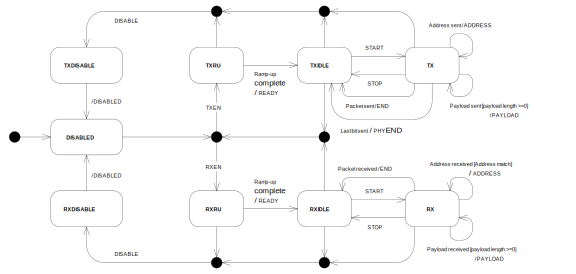
\includegraphics[width=1.0\textwidth]{nRF52840_Radio_states.png}
	\caption{Radio States \cite{nordic_semi_nrf_infocenter_radio_states_2020}}
	\label{fig:RadioStatesP2P}
\end{figure}

Die Radio Hardware der nRF52 und nRF53 SOCs verfügt über verschiedene Zustände (siehe Abbildung \ref{fig:RadioStatesP2P}). Abhängig von der gewünschten Operation (Senden oder Empfangen), werden die States abgearbeitet. Um Energie zu sparen wird nach Abschluss der gewünschten Tätigkeit immer in den Disabled-State gewechselt. Zusätzlich erfolgt das Benachrichtigen des Radio Drivers von der Hardware mittels Interrupts, wodurch der Energieverbrauch zusätzlich minimiert wird.

\begin{figure} [H]
	\centering
	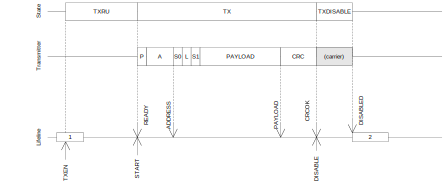
\includegraphics[width=1.0\textwidth]{nRF52840_Radio_Transmit_Sequence_with_Shorts.png}
	\caption{Sende-Ablauf mit Verknüpfungen \cite{nordic_semi_nrf_infocenter_radio_transmit_sequence_2020}}
	\label{fig:RadioTransmitSequP2P}
\end{figure}

Abbildung \ref{fig:RadioTransmitSequP2P} zeigt den Ablauf beim Senden eines Pakets. Die zu sendenden Daten (Payload) müssen vorgängig im RAM vorliegen. Anschliessend wird der Packet Pointer des Radio-Interface auf die entsprechende Speicher-Adresse eingestellt. Zu beachten gilt es das im ersten Byte die Länge der Payload angegeben sein muss. Diese wird vom Radio Driver automatisch ergänzt. Zusätzlich kann ein Adress-Feld den Sende-Daten mitgegeben werden. Nach dem vollständigen Konfigurieren des Radio-Interface wird das Senden durch den Befehl TXEN initiiert. Mithilfe von Verknüpfungen (Shorts) wird nach dem Ready-Event automatisch der Start-Task ausgelöst. Das Senden läuft also nach dem Initiieren vollautomatisch ab. Der Radio-Driver wartet lediglich auf das auslösen des Disabled-Events. Das Senden ist erfolgreich abgeschlossen und der Funktionsaufruf kehrt zum Hauptprogramm zurück. Das Senden mittels CCA wird im \textit{IEEE802.15.4-Mode} unterstützt. Dazu wird vor dem Senden der Kanal abgehört um Kollisionen zu vermeiden. Mittels dem RXEN Befehl wird der CCAStart-Task aktiv. Dieser führt abhängig vom Konfigurierten CCA-Modus eine Prüfung des Kanals durch. Ist der Kanal nicht belegt wird ein CCAIdle-Event generiert, welcher mittels Verknüpfung automatisch den TXEN-Task Startet (siehe Abbildung \ref{fig:CCAIDLEP2P}). Sendet ein andere Teilnehmer momentan auf dem Kanal wird ein CCABusy-Event generiert, welcher ebenfalls den Disable-Taks ausführt (siehe Abbildung \ref{fig:CCABUSYP2P}). Somit Enden beide Varianten (Idle und Busy) im Disabled-State, wobei beim einen keine Daten gesendet werden konnten. \cite{nordic_semi_nrf_infocenter_radio_transmit_sequence_2020}

\begin{figure}[!htbp]
	\begin{minipage}{0.49\textwidth}
		\centering
		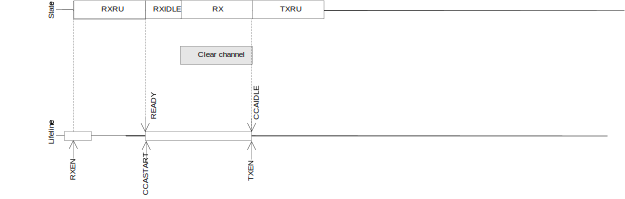
\includegraphics[width=\textwidth]{cca.png}
		\caption[Sende-Ablauf mit CCA Idle]{CCA Prüfung (Idle Event) \cite{nordic_semi_nrf_infocenter_radio_ieee_operation_2020}}
		\label{fig:CCAIDLEP2P}
	\end{minipage}
	\begin{minipage}{0.49\textwidth}
		\centering
		\includegraphics[width=\textwidth]{cca_busy.png}
		\caption[Sende-Ablauf mit CCA Busy]{CCA Prüfung (Busy Event) \cite{nordic_semi_nrf_infocenter_radio_ieee_operation_2020}}
		\label{fig:CCABUSYP2P}
	\end{minipage}
\end{figure}

\begin{figure} [H]
	\centering
	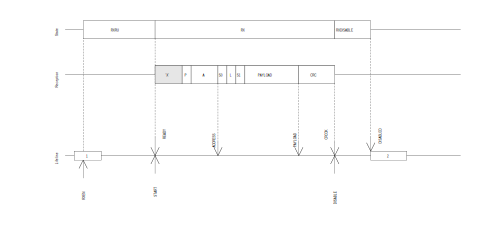
\includegraphics[width=1.0\textwidth]{nRF52840_Radio_Receive_Sequence_with_Shorts.png}
	\caption{Empfangs-Ablauf mit Verknüpfungen \cite{nordic_semi_nrf_infocenter_radio_receive_sequence_2020}}
	\label{fig:RadioReceiveSequP2P}
\end{figure}

Der Ablauf zum Empfangen eines Pakets wird in Abbildung \ref{fig:RadioReceiveSequP2P} dargestellt. Grundsätzlich ist der Ablauf gleich Aufgebaut wie beim Senden von einem Paket. Nach Initiieren mittels dem RXEN-Befehl fährt der Empfänger hoch und wartet auf den Empfang eines Pakets. Nach eingehen einer Preamble-Sequenz wird das Address-Feld geprüft. Dieses kann vorgängig festgelegt werden um nur Pakete mit übereinstimmender Adresse zu empfangen. Bei allen BLE-Modes erfolgt die Prüfung auf Hardware-Ebene (ohne Interaktion der CPU) ab. Beim \textit{IEEE802.15.4-Mode} steht dieses Feature nicht zur Verfügung. Das vergleichen des Adress-Feldes muss der Radio-Driver selbst übernehmen. Um die Signalstärke (RSSI) vom eingehenden Paket zu messen, wird eine Verknüpfung zwischen dem \textit{Address-Event} und dem \textit{RSSIStart-Task} aktiviert. Nach erfolgreichem Prüfen der CRC Checksumme wird mittels einer Verknüpfung des CRCOK-Event der Disable-Task ausgeführt. Beim Empfangen eines Pakets wartet der Radio-Driver während eines gewissen Timeouts auf den Disabled-Event. Die Empfangsfunktion gibt die Restzeit des Timeouts in Millisekunden zurück, wodurch sich ein erfolgreiches Empfangen prüfen lässt. Das Bufferhandling übernimmt der Radio-Driver und erwartet beim Senden und Empfangen von Daten eine vordefinierte \textit{Radio-Packet-Structure}. Zu beachten gilt es das die Daten erst nach dem End-Event  vollständig abgearbeitet wurden, da der Zugriff von der Hardware über DMA erfolgt. Ebenfalls wurde festgestellt das beim wechseln auf oder von dem \textit{IEEE802.15.4-Mode} der Kanalwechsel vor dem Modewechsel erfolgen muss. Ansonsten werden keine Pakete empfangen. \cite{nordic_semi_nrf_infocenter_radio_receive_sequence_2020}


\subsection{Broadcasting Collisions Probability}\label{sec:BroadcastingCollissionsProbability}

Kollisionen entstehen wenn mehrere Teilnehmer gleichzeitig auf dem selben Kanal (Frequenz) senden. Dabei stören sich die beiden Sender und es kann sein das der Empfänger keine Daten empfangen kann. Dies ist leider nicht immer zu vermeiden, zum Beispiel wenn sich mehrere Teilnehmer neu mit dem Netz verbinden möchten. Im Fall der P2P-Testinfrastruktur entsteht ein solcher Fall im Mockup-State. Hier soll sich jeder Slave, welcher dem Master noch unbekannt ist, auf die Discovery-Anfrage des Masters melden. Die Lösung ist das jeder Slave einen zufälligen Zeitpunkt zum Antworten auswählt. Doch wie lange muss das Zeitfenster sein in welchem ein Slave einen Zeitpunkt zufällig auswählen darf? \\

Angenommen es gibt $N$ Teilnehmer, welche $t_a$ Sekunden brauchen um eine Antwort zu Senden. Zusätzlich existieren $N_{ch}$ verschiedene Kanäle auf welchen die Teilnehmer antworten können. Die Wahrscheinlichkeit das sich zwei Sender nicht überlappen $P_{miss}$ im Zeitfenster $t_I$ Sekunden lässt sich gemäss Formel \ref{eq:BroadcastingMissProbability} bestimmen. \cite{rk_how_to_deal_with_broadcasting_collision_2020}

\begin{equation}\label{eq:BroadcastingMissProbability}
P_{miss} = (1- \frac{2 \cdot t_a}{N_{ch}} \cdot t_I)^{N-1}
\end{equation}

Die folgenden Werte wurden zur Berechnung des Zeitfensters im Mockup-State verwendet:

\begin{itemize}
	\item $N = 50$
	\item $t_a = 5ms$
	\item $N_{ch} = 3$
	\item $t_I = 1.2s$	
\end{itemize} 

Somit liegt die Wahrscheinlichkeit das alle 50 Nodes sich verfehlen bei 85\%. 

\subsection{Zeitsynchronisation}\label{sec:Zeitsynchronisation}

Die Zeitsynchronisation wurde mittels einer Offset Kompensation gelöst. Der Zeitgeber (Master) sendet seine Zeit (Timestamp) über einen Broadcast an alle Teilnehmer in der Umgebung. Die Slaves vergleichen den empfangene Master-Zeit mit ihrer lokalen Zeit und errechnen den Unterschied (Offset) zwischen dem Master-Timestamp und Slave-Timestamp. Somit können sie ihre Zeit mittels an die des Masters angleichen. Das Prinzip ist realtiv simpel birgt jedoch einige Ungenauigkeiten. Die Verzögerungszeit zwischen dem auslesen des Master-Timestamp bis zum empfangen und vergleichen mit dem Slave-Timestamp ist sehr relevant.  

\begin{figure} [H]
	\centering
	\includegraphics[width=1.0\textwidth]{Timesync_Basic.png}
	\caption{Zeitsynchronisation über Offset mit Fehler}
	\label{fig:TimesyncBasicwithErrorP2P}
\end{figure}

Wie in Abbildung \ref{fig:TimesyncBasicwithErrorP2P} ersichtlich entsteht beim Auslesen der Zeit bis zum Senden eine Verzögerung die TxChainDelay, sowie beim Empfänger die RxChainDelay. Da Ziel ist es diese Verzögerungen so gering wie möglich zu halten. 

\begin{figure} [H]
	\centering
	\includegraphics[width=1.0\textwidth]{Tiesync_Advanced.png}
	\caption{Zeitsynchronisation über Offset mit PPI}
	\label{fig:TimesyncwithPPIP2P}
\end{figure}

Die Lösung wird in Abbildung \ref{fig:TimesyncwithPPIP2P} gezeigt. Der nRF52840 SOC verfügt über ein PPI (Programmable peripheral interconnect). Mithilfe des PPI lassen sich verschiedene Events und Tasks direkt Verknüpfen, ohne das die CPU dabei involviert ist. Dies erlaubt uns das Erfassen des Zeitwerts (Task) mit dem Erfolgreichen Senden des "Probe Packets" (Event) zu verbinden. Dazu wurde der Timer-Capture-Task des Synctimers und der Radio-End-Event über ein PPI miteinander verknüpft. Beim Slave wird der Event das ein Packet erfolgreich Empfangen wurde (Radio-CRCOK-Event) mit dem Erfassen des Synctimers (Synctimer-Capture-Task) verknüpft. 


\todo[inline]{Wie wurde die Zeitsynchronisation umgesetzt? Wie relevant ist diese für die Messungen?}
\pagebreak

\clearpage
\section{Hardware Plattform}\label{sec:HardwarePlattform}
\todo[inline]{Cyrill}

\todo[inline]{Übersicht über die eingesetzte Hardware. Einleitung inkl. Erläuterung Unterschiede und Gemeinsamkeiten P2P und Mesh Test Hardware (Stichwort: Open Source, Open Hardware).}

\subsection{System on Chip}\label{sec:SystemonChip}
\todo[inline]{Kurze Beschreibung des nRF52840.}

\subsection{Hardware Development Kits}\label{sec:HardwareDevelopmentKits}
\todo[inline]{Kurze Beschreibung der nRF52840 DK's. Dongle und DK. Was wird wo eingesetzt?}

\subsection{Aufbau Testnode}\label{sec:AufbauTestnode}
\todo[inline]{Dongle mit Batteriehalter. Wie wird der Dongle geflasht? Benchmark Master mit einem DK umgesetzt.}

\subsection{Benchmark Management Station}\label{sec:BenchmarkManagementStation}
\todo[inline]{Raspberry Pi4}
\pagebreak

\clearpage
\section{Messungen Mesh Netzwerke}\label{sec:MessungenMeshNetzwerke}

\subsection{Messaufbau}\label{sec:Messaufbau}

\subsection{Ablauf}\label{sec:Ablauf}




\pagebreak

\clearpage
\section{Point to Point Testinfrastruktur}\label{sec:PointtoPointTestinfrastruktur}

\subsection{Messaufbau}\label{sec:Messaufbau}

\subsection{Ablauf}\label{sec:Ablauf}

\subsection{Aufbau und Bedienung der Messinfrastruktur}\label{sec:AufbauundBedienungderMessinfrastruktur}

\subsection{Interpretation der Messresultate für den Anwender}\label{sec:InterpretationderMessresultatefürdenAnwender}
\pagebreak

%%Part 1 Bluetooth Mesh

	\clearpage
\section{Übersicht}\label{sec:Uebersicht}

Das vorliegende Dokument stellt das Pflichtenheft der Bachelorthesen von Raffael Anklin, Robin Bobst und Cyrill Horath an der Fachhochschule Nordwestschweiz Brugg-Windisch im Studiengang Elektro- und Informationstechnik dar. 
Im kommenden ersten Kapitel soll eine Übersicht über die Ausgangslage sowie das Ziel dieser Arbeit gegeben und somit die Rahmenbedingungen abgesteckt werden. Weiter werden die Lösungskonzepte \ref{sec:Loesungskonzept} sowie die Projektziele und Lieferobjekte \ref{sec:ProjektzieleundLieferobjekte} definiert. Abschliessend soll auch noch das Projektmanagement \ref{sec:Projektmanagement} thematisiert werden. 

\subsection{Ausgangslage}\label{subsec:Ausgangslage}

Unter den standardisierten Low Power Mesh Netzwerk Protokollen im
freien GHz ISM-Band konkurrenzieren sich derzeit vorrangig Bluetooth Mesh, Zigbee sowie Thread.
Bezüglich MAC und Physical Layer basieren Zigbee und Thread auf IEEE 802.15.4 wogegen Bluetooth Mesh auf Bluetooth Low Energy (BLE)
basiert.
Jedes dieser Netzwerkprotokolle hat gewisse Vorzüge: Bluetooth Mesh, dass BLE mittlerweile von jedem Smartphone und Notebook unterstützt wird, Thread aufgrund seiner IPv6 Basis und damit einfachem Übergang ins Internet sowie Zigbee aufgrund seiner etablierten Verbreitung im Smart-Lampenbereich durch Philips, IKEA und Osram.
Hauptproblem aller drei Mesh Netzwerkprotokolle ist nebst physikalisch und distanzbedingter Absorption und Reflexion die Störbeeinflussung durch WLAN (WiFi) und andere Netzwerke im GHz Frequenzbereich.

Im Rahmen des P5 mit dem Namen \textit{Bluetooth-Mesh Plattform für IoT Anwendungen}, wurde das Bluetooth-Mesh Protokoll bereits vertieft betrachtet und dessen Vor- und Nachteile aufgezeigt. Basierend auf diesen Erkenntnissen und Erfahrungen und der oben beschriebenen Thematik soll das Bluetooth-Mesh Protokoll mit den Alternativen Thread sowie Zigbee verglichen werden.

\subsection{Ziel der Arbeit}\label{subsec:ZielderArbeit}

In der vorliegenden Arbeit soll zuerst ein praxistaugliches, einheitliches Testframework für alle drei Mesh Netzwerke erstellt werden, wonach die Tauglichkeit aller drei Mesh Netzwerke unter realitätsnahen Bedingungen ermittelt und verglichen werden soll.
Zwecks besserer Vergleichbarkeit sollen alle drei Testnetze das gleiche Radio-Interface als Grundlage verwenden. Aufgrund der guten
Unterstützung aller drei Mesh Protokolle als auch dem im vergangenen P5 gesammelten Wissens, sollen hierfür die nRF52840 SoCs der Firma Nordic eingesetzt werden. Die zu erstellende Testinfrastruktur soll aus den drei folgenden Teilen bestehen:

\begin{itemize}
 	\item Punkt-Punkt Testinfrastrukturen auf MAC-Ebene
 	\item Test Mesh Netzwerke für BT Mesh, Zigbee und Thread
 	\item Steuer- und Auswertesoftware
\end{itemize}

Die genauen Anforderungen an die Testumgebung sind einerseits in der Aufgabenstellung im Anhang \ref{app:Aufgabenstellung} aufgeführt und andererseits werden sie anhand der Projektziele \ref{sec:ProjektzieleundLieferobjekte} definiert.









\pagebreak

\clearpage
\section{Technische Grundlagen Bluetooth Mesh}\label{sec:TechnischeGrundlagenBluetoothMesh}




\subsection{Netzaufbau und Topologie}\label{sec:NetzaufbauundTopologie}

Nebst dem funktionellen Aspekt übernehmen Nodes unterschiedliche Rollen im Netzaufbau. Ein Node wird als Relay-Node bezeichnet. wenn dieser Nachrichten an weitere Teilnehmer weiterleitet. Ein Friend-Node dient als Zugangspunkt für einen Low-Power-Node. Der Low-Power-Node wird dort eingesetzt wo keine konstante Stromversorgung zur Verfügung steht. Dieser geht eine Beziehung mit einem Friend-Node ein. Der Friend-Node speichert alle Nachrichten der LPNs, welche mit ihm eine Beziehung pflegen. In einem festen Zeitintervall fragt der LPN die verpassten Nachrichten beim Friend-Node ab. Dadurch kann der LPN zwischen Abfragen inaktiv bleiben um Energie zu sparen. Um die Interoperabilität zwischen inkompatiblen Bluetooth-Mesh Geräten und einem Mesh-Netzwerk zu ermöglichen existieren Proxy-Nodes. Ein Proxy-Node dient als Schnittstelle in das Netzwerk und erlaubt das Interagieren über Bluetooth-GATT mit dem Mesh. Dies ermöglicht das steuern des Netzwerks über das Smartphone. Die in Abbildung \ref{fig:BTMeshTopology} gezeigt Topologie zeigt die verschiedenen Node-Typen an ihrem Einsatzort. 

\begin{figure} [H]
	\centering
	\includegraphics[width=1.0\textwidth]{Bluetooth_Mesh_Topology.PNG}
	\caption{Beispielhafte Topologie eines Bluetooth-Mesh Netzwerks \cite{bluetooth_sig_mesh_netzwerk_spezifikationen_2020}} 
	\label{fig:BTMeshTopology}
\end{figure}


\subsection{Protokoll Stack}\label{sec:BLEMeshProtokollStack}
In diesem Abschnitt wird die Architektur des Mesh-Stacks genauer untersucht. Der Grundsätzliche Aufbau wird Abbildung \ref{fig:BTMeshStack} veranschaulicht. Eine Grafik zur Veranschaulichung des Message-Flows durch die einzelnen Schichten ist im Anhang \ref{app:BluetoothMeshStackLayers} ersichtlich. 

Wie in Kapitel \ref{sec:EinleitungBluetooth} bereits erwähnt basiert der Stack auf Bluetooth Low Energy. Der BLE-Layer dient zur Grundlegenden Schicht des Stacks. Der Zugriff für Mesh-Traffic erfolgt über das GAP-Profil, der für Proxy Traffic über das GATT-Profil. Der Bearer-Layer regelt den Zugriff auf den BLE-Stack. Es existieren verschiedene Bearers. Der GATT-Bearer ermöglicht Geräten ohne GAP Zugriff auf das Netzwerk. Der Advertising-Bearer wird für den Mesh-Traffic benutzt. 

Der Network-Layer hat folgende Aufgaben zu erfüllen: 

\begin{itemize}
	\item Ver- und Entschlüsselung der Network-PDU
	\item Filtern von nicht relevanten Nachrichten (Adressauflösung)
	\item Relaying von Paketen mittels TTL-Field
\end{itemize}

\begin{wrapfigure}{r}{0.5\textwidth}
	\centering
	\includegraphics[width=0.5\textwidth]{Bluetooth_Mesh_Stack_Layers.PNG}
	\caption{Bluetooth-Mesh Stack \cite{bluetooth_sig_mesh-technology-overviewpdf_2020}} 
	\label{fig:BTMeshStack}
\end{wrapfigure}

Zudem bedient dieser Layer verschiedene Bearers und ist dafür verantwortlich das alle relevanten Pakete zur entsprechenden Stelle weitergeleitet werden.

Über dem Network Layer befindet sich der Transport-Layer, welcher in einen Lower- und Upper-Transport-Layer aufgeteilt ist. Der Lower-Transport-Layer handelt das Acknowledgement einzelner Segmente von eingehenden Nachrichten ab. Zudem beeinhaltet er das Herz-Stück des Friend-Features, nämlich die Friend-Queue. In diesem Buffer werden alle Nachrichten der  Low-Power-Nodes aufbewahrt. Ebenfalls führt diese Schicht das Segmentieren und Zusammensetzen der Pakete (SAR) durch. Pakete werden in Fragmente aufgeteilt, welche lediglich 8-10 Byte an Applikations-Daten beherbergen können.

Der Upper-Transport-Layer dient hauptsächlich zur Ver- und Entschlüsselung von Paketen auf Transport-Ebene. Zudem werden Anfragen wie Friend-Requests über diese Schicht verarbeitet.

Der Access-Layer führt die Zuordnung der Nachrichten an die Models durch. Diese Schicht regelt den Zugriff der Applikation auf die unterliegenden Schichten. Zudem werden Nachrichten auf allfällige Replay-Messages geprüft, bevor sie an die Applikation weitergegeben werden.

Die zweitletzte Schicht bildet der Foundation-Models-Layer. Seine Aufgabe ist es die Models zu Verwalten, welches über das Config-Server-Model geschieht. Zusätzlich gehört ein Health-Model zu den Foundation-Models, welches den Zustand des Teilnehmers überwacht. Beide Models müssen zwingend auf jedem Node vorhanden sein. \cite{bluetooth_sig_mesh_netzwerk_spezifikationen_2020} \cite{bluetooth_sig_mesh-technology-overviewpdf_2020}

Als letzte Schicht dienen die Models. Dessen Funktionalität ist rein von der Applikation abhängig (siehe Abschnitt \ref{sec:EinleitungBluetooth}). Daher kann diese Schicht als Application-Layer aufgefasst werden.


\subsection{Sicherheit}\label{subsec:BleutoothMeshSicherheit}
Bleutooth-Mesh Nachrichten werden zweifach Verschlüsselt. Die Network-PDU ist mit dem zugehörigen Network-Key gesichert. Wer im Besitz des Netzwerk-Schlüssels gelangt, kann Nachrichten bis zum Upper-Transport-Layer auslesen. Für Teilnehmer welche die Nachricht nur weiterleiten (Relayen) müssen, reicht dieser Einblick aus. Auf Applikationsebene findet die Verschlüsselung zusätzlich über einen Application-Key statt. Nur Teilnehmer mit dem richtigen Applikation-Key können an Informationen der Models gelangen und diese Steuern.

Zusätzlich zur Verschlüsselung führt jeder Teilnehmer eine fortlaufenden Nummerierung der Nachrichten durch (SEQ-Field). Damit lassen sich sogenannte Replay-Attacks verhindern.

Um während des Provisioning-Ablauf die Authentifizierung des neuen Teilnehmers sicher zu Stellen, wird ein Device-Key verwendet. Dieser dient einmalig dazu das neue Gerät einzubinden und zu konfigurieren. 



\subsection{Bluetooth Mesh Software Development Kit}\label{sec:BluetoothMeshSoftwareDevelopmentKit}
Die Umsetzung des Bluetooth-Mesh-Stacks ist für die nRF-Platform mittels den folgenden zwei Bibliotheken möglich. 

\begin{itemize}
	\item \textit{\textbf{nRF Connect SDK}}: Auf dem Zephyr-RTOS aufbauende SDK. Zephyr Implementation des Mesh-Stacks, welche von Bluetooth SIG anerkannt ist. Von Nordic nicht zur Verwendung in Endprodukten empfohlen. Unterstützt neuere SOCs wie den nRF5340.  \cite{nordic_semi_welcome_to_the_nrf_connect_sdk_2020}
	\item \textit{\textbf{nRF SDK for Mesh}}: Proprietäre SDK Library von Nordic Semiconductor für Bluetooth-Mesh. Ist zum Einsatz in Endprodukten freigegeben. \cite{nordic_semi_nrf_sdk_for_mesh_2020}
\end{itemize}

Da der neuere SOC nur von der nRF Connect SDK unterstützt wird, sowie die Zephyr Implementation auf weitere SOCs andere Hersteller anwendbar ist, wurde die Implementation mit dieser Bibliothek vorangetrieben. Als Nebenprodukt wurde die Entwicklung mit der nRF SDK for Mesh ins Auge gefasst um die beiden SDKs miteinander zu vergleichen. Zu diesem Zeitpunkt ist ein direkter Vergleich leider noch nicht möglich, da die Funktionalität der nRF SDK for Mesh Variante noch nicht vollständig umgesetzt wurde. Die Umsetzung des Benchmarks wird im folgenden Abschnitt dokumentiert.


\pagebreak

\clearpage
\section{Firmware Benchmark}\label{sec:FirmwareBenchmark}

\subsection{Benchmark Master}\label{sec:BenchmarkMasterBluetooth}


\subsection{Benchmark Server}\label{sec:BenchmarkServerBluetooth}


\subsection{Benchmark Client}\label{sec:BenchmarkClientBluetooth}

\pagebreak


%%Part 2 Thread

\vspace*{4cm}
\begin{center}
\part{Thread}
\end{center}
\vspace*{\fill}
\clearpage

\section{Übersicht}\label{sec:Uebersicht}








\pagebreak

\clearpage
\section{Technische Grundlagen Thread}\label{sec:TechnischeGrundlagenThread}

\subsection{Netzaufbau und Topologie}\label{subsec:NetzaufbauundTopologie}
\todo[inline]{Welchen Aufbau? Welche Art von Mesh? Welche Nodetypen gibt es? Welche typischen Eigenschaften besitzt das Protokoll?}
\subsubsection{Node Typen}\label{subsubsec:NodeTypen}
\textbf{Full Thread Device (FTD)}

\underline{Leader:}

\underline{Router:}

\underline{Full End Device:}

\textbf{Minimal Thread Device (MTD)}

\underline{Minimal End Device:}

\underline{Sleepy End Device:}

\subsubsection{IPv6 Adressierung}\label{subsubsec:IPv6Adressierung}

\subsubsection{Netzwerk Aufbau}\label{subsubsec:NetzwerkAufbau}

\subsubsection{Router Auswahl}\label{subsubsec:RouterAuswahl}

\subsection{Thread Protokoll Stack}\label{subsec:ThreadProtokollStack}
\todo[inline]{Erläuterung des Protokoll Stacks. Möglichst viel Grafiken und nur so viel als nötig Prosa.}

\subsection{Thread Software Development Kit}\label{subsec:ThreadSoftwareDevelopmentKit}
\todo[inline]{Eingesetzte SDK und deren Aufbau beschreiben. Allenfalls die wichtigsten API Funktionen genauer erläutern.}

\pagebreak

\clearpage
\section{Umsetzung Benchmark}\label{sec:ThreadUmsetzungBenchmark}
\todo[inline]{Einleitung schreiben}

\subsection{Openthread Stack Konfiguration}\label{subsec:ThreadStackKonfiguration}
\todo[inline]{Konfig erklären}
\begin{table}[h]
	\centering
	\begin{adjustbox}{width=1\textwidth}
		\begin{tabular}{lll}
			Stack Init Time                            & 30000 ms                                                               & \begin{tabular}[c]{@{}l@{}}Zeit die benötigt wird um den Stack für den Benchmark\\zu initialisieren. Reserve Zeit um das Routing des \\Netzwerkes durchzuführen.\end{tabular}  \\
			IEEE Channel                               & 15                                                                     & Thread Kanal der verwendet wird um das Mesh aufzubauen.                                                                                                                        \\
			Netzwerk Name                              & OpenThread                                                             & Netzwerkname~                                                                                                                                                                  \\
			\textcolor[rgb]{0.278,0.278,0.278}{PAN ID} & \textcolor[rgb]{0.278,0.278,0.278}{0xABCD}                             & Wird für das Precomissioning verwendet.                                                                                                                                        \\
			Netzwerkschlüssel                          & \textcolor[rgb]{0.278,0.278,0.278}{0x00112233445566778899AABBCCDDEEFF} & Wird für das Precomissioning verwendet.                                                                                                                                       
		\end{tabular}
	\end{adjustbox}
	\caption{Messgrössen Gewinnung und Verwendung}
	\label{tab:ThreadMessgrössenGewinnungundVerwendung}
\end{table}

\todo[inline]{bm\_config.h}

\todo[inline]{bm\_ot.c}

\subsection{CoAP Benchmark Message}\label{subsec:ThreadBenchmarkMessage}
\todo[inline]{CoAP erklären}

\subsection{IPv6 Adressierung}\label{subsec:IPv6Adressierung}
\todo[inline]{IPv6 group multicast erklären}
\pagebreak



%%Part 3 Zigbee

\vspace*{4cm}
\begin{center}
\part{Zigbee}
\end{center}
\vspace*{\fill}
\clearpage

\section{Übersicht}\label{sec:Uebersicht}








\pagebreak

\clearpage
\section{Technische Grundlagen Zigbee}\label{sec:TechnischeGrundlagenZigbee}

\subsection{Netzaufbau und Topologie}\label{subsec:ZigbeeNetzaufbauundTopologie}
Zigbee ist nicht gleich Zigbee.
Obschon Zigbee von der zentralen Stelle der Zigbee Alliance spezifiziert wurde, gibt es eine Vielzahl an Versionen und Umsetzungsvarianten.
In den Spezifikationen der Zigbee Alliance wird zwischen zwei sogenannten Stackprofilen \textit{ZigBee} und \textit{ZigBee PRO} unterschieden.
Während \textit{ZigBee}-Netzwerke eine Baumstruktur bilden und der Koordinator dabei einen Single-Point-of-Failure darstellt, haben \textit{ZigBee PRO}-Netzwerke geroutete Mesh Funktionalitäten mit Routing Tabellen und Wegentdeckung.
Der Koordinator bildet dabei nicht länger einen Single-Point-of-Failure, da sich das Routing dynamisch anpassen kann.
Abbildung \ref{fig:NetzwerktopologienZigbee} zeigt die Unterschiede eines Baumnetzwerks im Stackprofil \textit{ZigBee} links, und eines Meshnetzwerks im Stackprofil \textit{ZigBee PRO} rechts.
In der vorliegenden Arbeit wurde ausschliesslich das \textit{ZigBee PRO}-Stackprofil verwendet, womit vollwertige Meshnetzwerke möglich sind.

\begin{figure}[h]
	\centering
	\includegraphics[width=0.8\textwidth]{Zigbee_Netztopologie.png}
	\caption{Zigbee Baumnetzwerk links und Meshnetzwerk rechts \cite[S.~221]{markus_krause_rainer_konrad_zigbee_2014}}	\label{fig:NetzwerktopologienZigbee}
\end{figure}

Wie in Abbildung \ref{fig:NetzwerktopologienZigbee} bereits angedeutet, kann innerhalb eines Zigbee Meshnetzwerkes zwischen drei Node Rollen unterschieden werden. Diese besitzen unterschiedliche Aufgaben und Eigenschaften und sind wie nachfolgend beschrieben, spezifiziert:

\paragraph{Zigbee Koordinator}
Als zentrale Einheit übernimmt der \textit{Zigbee Koordinator}, Aufgaben wie den Aufbau und die Verwaltung eines WPAN (Wireless Personal Area Network) inkl. der Definition der wichtigsten Parameter, wie der PAN-ID, den Sicherheitsschlüsseln sowie der Wahl des IEEE Channels.
In einem Zigbee-Netzwerk gibt es genau ein Gerät das die Rolle des \textit{Zigbee Koordinators} einnimmt.
Welches diese ist, wird vom Anwender respektive Entwickler bestimmt.
Wenn dieses Gerät das Netzwerk verlässt oder kurzzeitig ausser Betrieb ist, kann das Netzwerk weiter bestehen und wie bisher betrieben werden.
Für die Aufnahme von zusätzlichen Nodes oder um beispielsweise die Sicherheitsschlüssel zu aktualisieren, muss der Koordinator wieder mit dem Netz verbunden werden.
Jeder \textit{Zigbee-Koordinator} besitzt gleichzeitig auch die Rolle eines \textit{Zigbee-Router}. \cite{markus_krause_rainer_konrad_zigbee_2014}

\paragraph{Zigbee Router}
\textit{Zigbee-Router} bilden das eigentliche Meshnetzwerk wie es in Abbildung \ref{fig:NetzwerktopologienZigbee} schematisch dargestellt ist.
Sie übernehmen die Aufgabe des Routings und leiten Pakete innerhalb des Netzwerkes weiter.
Durch Wegentdeckungsanfragen, werden Routing-Tabellen aufgebaut und fortlaufend aktualisiert.
Diese Routing-Tabellen sind entscheidend für den gerouteten Versand von Datenpaketen.
\textit{Zigbee-Router} sind zudem potentielle Zugriffspunkte zum Netzwerk für \textit{Zigbee End-Devices}. \cite{markus_krause_rainer_konrad_zigbee_2014}

\paragraph{Zigbee End-Device}
Die einfachste Rolle in einem Zigbee Netzwerk ist jene des \textit{Zigbee End-Device}. \textit{Zigbee End-Devices} stehen in einer Parent-Child Beziehung mit einem \textit{Zigbee-Router}.
Diese Kommunikation findet entweder periodisch oder ausgelöst durch einen Userinput statt.
Ankommende Pakete werden jeweils vom Parent-Node gespeichert bis das \textit{Zigbee End-Device} diese abruft.
\textit{Zigbee End-Devices} besitzen ausserdem keine Routing Funktionen und gelten deshalb als sehr energiesparend.
Ausgeführt als \textit{Sleepy-End-Device} können CPU und RAM des entsprechenden Nodes ganz oder teilweise heruntergefahren und durch periodische Interrupts geweckt werden.
Dadurch können noch längere Batteriestandzeiten erreicht werden.
In der Anwendung werden beispielsweise Lichtschalter als \textit{Sleepy-End-Device} ausgeführt die keine draht­ge­bun­dene Energieversorgung besitzen. \cite{markus_krause_rainer_konrad_zigbee_2014}


\subsection{Zigbee Protokoll Stack}\label{subsec:ZigbeeProtokollStack}
Die Architektur des Zigbee Stacks besteht aus vier Layern, dem Physical Layer (PHY), dem Media Access Control Layer (MAC), dem Network Layer (NWK) und dem Application Layer (APL).
Abbildung \ref{fig:ArchitekturdesZigbeeProtokollStacks} zeigt den Aufbau des Protokoll Stacks.
Jede der Schichten ist mit bestimmten Aufgaben betraut und stellt der darüber liegenden Schicht die notwendigen Daten und Dienste bereit.
Nachfolgend wird auf die vier Schichten des Zigbee Stacks eingegangen und deren Aufgabe und Funktionsweise kurz erläutert.

\begin{figure}[h]
	\centering
	\includegraphics[width=0.6\textwidth]{Zigbee_Architektur.png}
	\caption{Architektur des Zigbee Protokoll Stacks}
	\label{fig:ArchitekturdesZigbeeProtokollStacks}
\end{figure}

\subsubsection{MAC und PHY Layer}\label{subsubsec:MACundPHYLayer}
Der MAC wie auch der PHY Layer werden im Zigbee Protokoll Stack gebildet durch den \textit{IEEE 802.15.4} Standard für \textit{Wireless Personal Area Networks (WPAN)}.
Während beispielsweise Wifi oder Bluetooth, die auf dem selben 2.4 GHz ISM-Funkfrequenzband betrieben werden können, für hohe Datenübertragungsraten konzipiert wurden, ist dieser Standard für kleinere Datenmengen optimiert.
Durch die Vermeidung von unnötigen Steuerinformationen, kann der \textit{IEEE 802.15.4} Standard auf einfachster Hardware realisiert und mit kleinstem Energieaufwand betrieben werden.
Dies ist ideal für sogenannte \textit{Wireless Sensor Networks (WSN)}.
Zigbee ist nur eines von vielen Protokollen die diesen Standard benutzen.
MAC und PHY Layer sind für die physikalische Datenübertragung von einem Node zum Anderen zuständig.
Dazu besitzt jedes Funkmodul eine einmalige 48-Bit MAC Adresse mit welcher das Gerät eindeutig identifiziert und adressiert werden kann. \cite{markus_krause_rainer_konrad_ieee_2014}


\subsubsection{Network Layer (NWK)}\label{subsubsec:Network Layer}
Der NWK Layer ist im Zigbee Stack verantwortlich für den Aufbau sowie das Management der Netzwerkfunktionen und das Routing innerhalb dieses Netzwerkes.
Im NWK Layer wird das eigentliche Mesh gebildet und unterhalten. Dazu gehören die beiden Hauptaufgaben \textit{Netzaufbau und Adressierung} sowie das \textit{Routing}.

\paragraph{Netzaufbau und Adressierung}
Wie unter \ref{subsec:ZigbeeNetzaufbauundTopologie} bereits erwähnt, ist der Koordinator verantwortlich für den Aufbau des Zigbee Netzwerks und der Wahl von entsprechend geeigneten Parametern.
Dazu gehört beispielsweise eine 16-Bit PAN-ID sowie die Wahl eines möglichst störungsfreien Funkkanals.
Beim Beitritt eines neuen Funkmoduls, wird diesem durch den Koordinator eine im Netzwerk einmalige 16-Bit \textit{Short-Address} zugewiesen.
Anhand dieser kann das Funkmodul nun im Netzwerk adressiert werden und es selbst kann damit Routing Funktionen wahrnehmen.
Die im MAC Layer definierte 48-Bit MAC Adresse wird im NWK Layer zu einer statischen 64-Bit \textit{Long-Address} gewandelt.
Diese kann im Zigbee Stack ebenfalls für die Adressierung verwendet werden.
In einer \textit{Address-Table} sind die statischen \textit{Long-Addresses} und die dynamischen \textit{Short-Addresses} einander eindeutig zugewiesen.
Für die Adressierung im NWK Layer und für das Routing wird ausschliesslich die \textit{Short-Address} verwendet.

\paragraph{Routing}
Innerhalb von Zigbee Mesh Netzwerken, welche das \textit{ZigBee PRO} Stackprofil verwenden, werden durch jeden \textit{Zigbee-Router}, Routingtabellen erstellt.
Falls sich das Netzwerk verändert, werden auch diese Routing-Tabellen nachgeführt.
In den Routing-Tabellen ist die \textit{Short-Address} des Zielnodes sowie die zugehörige \textit{Next-Hop-Address} zum Ziel hinterlegt.
Eine zentrale Einheit die das Routing übernimmt gibt es dementsprechend nicht.
Enthält die Routingtabelle veraltete Einträge oder sind für das entsprechende Ziel noch keine Informationen vorhanden, muss ein \textit{Route Discovery} durchgeführt werden.
Hierbei handelt es sich um eine Broadcast Nachricht welche an alle Router gesendet wird.
Die Router in unmittelbarer Umgebung empfangen die Nachricht und leiten sie, wiederum als Broadcast, an alle Router in ihrer Reichweite weiter.
Dabei werden die Wegkosten jeweils addiert um diese, sobald die Nachricht beim Zielnode angekommen ist, dem Absender mitzuteilen.
So wird der Weg mit den geringsten totalen Wegkosten ermittelt und in der Routingtabelle abgelegt.


\subsubsection{Application Layer (APL)}\label{subsubsec:ApplicationLayer}
Der Zigbee Application Layer kann in drei Teile unterteilt werden, den Application Support Sublayer, das Zigbee Device Object und das Application Framework mit der Zigbee Cluster Library in der die eigentliche Anwendung definiert ist.

\paragraph{Application Support Sublayer (APS)}
Wie der Name andeutet ist der APS Layer für die Anwendungsunterstützung zuständig und als Zwischenschicht im Application Layer eingebettet.
Zu den Aufgaben des APS Layers gehören das \textit{Binding}, das \textit{Group-Management}, die Datenübertragung inkl. Fragmentierung sowie die Erstellung und der Versand von APS-Frames.
Ausserdem bietet der APS Layer eine Möglichkeit der Empfangsbestätigung auf Applikationsebene.
Anders als die Empfangsbestätigung auf MAC Ebene ist diese nicht nur auf Funkmodule in unmittelbarer Reichweite beschränkt.

\begin{figure}[h]
	\centering
	\includegraphics[width=\textwidth]{Zigbee_Frame_Structure.png}
	\caption{Zigbee Frame Struktur bei aktivierten Sicherheitsfunktionen \cite[S.~286]{markus_krause_rainer_konrad_zigbee_2014}}
	\label{fig:ZigbeeFrameStruktur}
\end{figure}

Die Fragmentierung von APS Nutzdaten basiert darauf, dass die Grösse von Frames durch den PHY Layer auf 127 Byte beschränkt ist.
Abzüglich sämtlicher Header auf MAC, NWK sowie APS Ebene und sonstigem Overhead des Protokolls, beispielsweise für Sicherheitsfunktionen (siehe Abschnitt \ref{subsucsec:ZigbeeSicherheit}), reduziert sich die nutzbare APS-Payload Grösse auf 53 Byte. In Abbildung \ref{fig:ZigbeeFrameStruktur} ist die Struktur eines kompletten Zigbee Frames dargestellt.
Sollen nun grössere Daten übertragen werden, führt der APS Layer eine Fragmentierung durch \cite[S.~279 - 299]{markus_krause_rainer_konrad_zigbee_2014}.


\paragraph{Application Framework (AF) mit Zigbee Cluster Library (ZCL)}
Das Application Framework bildet den Bereich des APL in dem die eigentliche Anwendung abläuft. Für die Adressierung stehen dem Anwender dabei 240 sogenannte Endpoints zur Verfügung. Endpoints können mit dem Prinzip von Ports im TCP/IP Modell verglichen werden.
Sie dienen dazu unterschiedliche Anwendungen auf dem selben Node zu adressieren.
Innerhalb des AF können Anwendungen nun prinzipiell frei umgesetzt werden.
Um den Anwendern jedoch eine herstellerunabhängige Plattform bieten zu können, wurde durch die Zigbee Alliance die \textit{Zigbee Cluster Library (ZCL)} spezifiziert.
Anwendungen wie beispielsweise ein Lichtschalter oder eine Lampe, werden durch sogenannte Cluster detailliert beschrieben.
Dabei handelt es sich um eine Sammlung von Kommandos und Attributen für den jeweiligen Anwendungszweck. \cite{the_zigbee_alliance_zigbee_2016}

\paragraph{Zigbee Device Object (ZDO)}
Das Zigbee Device Object ist ein eigenständiges Anwendungsobjekt welches immer mit dem Endpoint 0 addressiert wird.
Es setzt die Funktionalitäten gemäss Definition der Zigbee Rollen (Koordinator, Router, End-Device) um, und benutzt dafür Funktionen der NWK sowie APS Schicht.
Beispielsweise ist es zuständig für das Netzwerkmanagement, Knotenmanagement und auch für die Implementation von Sicherheitsfunktionen.

\subsubsection{Sicherheit}\label{subsucsec:ZigbeeSicherheit}
Die drahtlose Übertragung in einem WPAN ist vom Grundsatz her anfälliger für Angriffe oder Manipulationen wie eine drahtgebun­dene Kommunikation.
Deshalb ist die Implementation von Sicherheitsfeatures in einem \textit{Low Power Mesh Network} von grosser Bedeutung.
Zigbee verwendet ein \textit{CCM\footnote{Counter mode encryption and Cipher block chaining Message authentication code}} Verfahren auf MAC wie auch auf NWK und APS Ebene.
Dieses ist vom \textit{IEEE 802.15.4} Standard für die Verschlüsselung und Authentifizierung spezifiziert.
\textit{CCM} ist ein Verfahren für eine mehrmalige Blockverschlüsselung welches mit einem einzigen Schlüssel auskommt.
Das Verfahren nutzt den \textit{AES\footnote{Advanced Encryption Standard}}-Verschlüsselungsalgorithmus als Blockverschlüsselung.

\paragraph{Sicherheitsstufen}
Im \textit{CCM} Verfahren können 8 verschiedene Sicherheitsstufen gemäss Tabelle \ref{tab:SicherheitsstufeninZigbee} definiert werden.
Die Sicherheitsstufe 0 deaktiviert sämtliche Sicherheitsfunktionen.
Die Stufen 1 bis 3 fügen dem MAC Frame eine \textit{MIC\footnote{Message Integrity Code}} Prüfsumme von steigender Grösse hinzu, wodurch die Grösse des Frames zunimmt.
Erst ab Stufe 4 werden die Nutzdaten des MAC-Frames verschlüsselt und die Stufen 5 bis 7 mit einer \textit{MIC} Prüfsumme ergänzt. \cite[S.~334]{markus_krause_rainer_konrad_zigbee_2014}

\begin{table}[h]
\centering
\begin{tabular}{lll} 
\toprule
Sicherheitsstufe: & Verschlüsselung: & Authentifikation: \\ 
\hline
0 & Nein & Nein \\
1 & Nein & 32-Bit \textit{MIC} \\
2 & Nein & 64-Bit~\textit{MIC} \\
3 & Nein & 128-Bit~\textit{MIC} \\
4 & Ja & Nein \\
5 & Ja & 32-Bit~\textit{MIC} \\
6 & Ja & 64-Bit~\textit{MIC} \\
7 & Ja & 128-Bit~\textit{MIC} \\
\bottomrule
\end{tabular}
\caption{Sicherheitsstufen in Zigbee \cite[S.~334]{markus_krause_rainer_konrad_zigbee_2014}}
\label{tab:SicherheitsstufeninZigbee}
\end{table}

\paragraph{Schlüssel}
Für das \textit{CCM} Verfahren in Zigbee Netzwerken, werden zwei verschiedene Schlüsseltypen eingesetzt, der Netzwerkschlüssel und sogenannte Linkschlüssel.
In einem Zigbee Netzwerk mit normalem Sicherheitsmodus\footnote{Die Alternative zum Normalen Sicherheitsmodus wäre der Hohe Sicherheitsmodus. \cite[S.~338]{markus_krause_rainer_konrad_zigbee_2014}} wird einem Node die Rolle des \textit{Trustcenters} zugeordnet.
Üblicherweise übernimmt diese Rolle der \textit{Zigbee-Koordinator}.
Der Trustcenter-Node ist zuständig für die Verteilung der Sicherheitsschlüssel.
Beim Beitritt eines Nodes zum Netzwerk, überträgt das \textit{Trustcenter} den Netzwerkschlüssel über einen unverschlüsselten Kanal.
Dieser Netzwerkschlüssel wird nun für die Kommunikation zwischen Node und \textit{Trustcenter} benutzt.
Um Angriffe zu verhindern, wird der Netzwerkschlüssel durch das \textit{Trustcenter} regelmässig erneuert.
Dazu werden sogenannte Schlüsselwechsel-Kommandoframes versendet.
Für die Verschlüsselung von End-zu-End Verbindungen auf APS Ebene werden die Linkschlüssel eingesetzt, welche nur über die bereits gesicherte Verbindung vom Trustcenter zum Node übertragen werden.
Diese Linkschlüssel sind nur den beteiligten Nodes bekannt und werden üblicherweise durch das \textit{Trustcenter} ausgestellt.
Eine Alternative dazu wäre, dass die Linkschlüssel auf den entsprechenden Funkmodulen bereits vorinstalliert sind.


\pagebreak

\clearpage
\section{Umsetzung Benchmark}\label{sec:ZigbeeUmsetzungBenchmark}
\todo[inline]{Komplette Beschreibung der Firmware unterteilt in die 3 Nodetypen. Besonderheiten herausstreichen und allfällige Schwierigkeiten aufzeigen.}

\subsection{Benchmark und Stack Parameter}\label{subsec:BenchmarkundStackParameter}


\begin{table}[h]
\centering
\begin{adjustbox}{width=1\textwidth}
\begin{tabular}{lll}
Stack Init Time & 60000 ms & \begin{tabular}[t]{@{}l@{}}Zeit die benötigt wird um den Stack für den Benchmark\\zu initialisieren. Das Zigbee Netzwerk benötigt eine\\gewisse Zeit um sich aufzubauen\end{tabular} \\
IEEE Channel & 15 & Zigbee Kanal der verwendet wird um das Mesh aufzubauen. \\
Client Endpoint & 1 & Nummer für den Client Endpoint im ZCL Level Cluster \\
Server Endpoint & 10 & Nummer für den Server Endpoint im ZCL Level Cluster \\
Group ID & 0xB331 & \begin{tabular}[t]{@{}l@{}}Default Group ID. Zu diesem Wert wird der Index für die\\zugewiesene Gruppe addiert um die\\Gruppenzugehörigkeit festzulegen.\end{tabular}
\end{tabular}
\end{adjustbox}
\caption{Messgrössen Gewinnung und Verwendung}
\label{tab:MessgrössenGewinnungundVerwendung}
\end{table}

\subsection{Mesh Node Firmware}\label{subsec:ZigbeeMeshNodeFirmware}

\subsubsection{Stack Configuration}\label{subsubsec:ZigbeeStackConfiguration}

\todo[inline]{bm\_config.h}

\subsubsection{Stack Handling}\label{subsubsec:ZigbeeStackHandling}

\todo[inline]{bm\_zigbee.c}

\paragraph{Master}\label{par:ZigbeeMaster}

\paragraph{Client}\label{par:ZigbeeClient}

\paragraph{Server}\label{par:ZigbeeServer}


\subsection{Benchmark Message}\label{subsec:BenchmarkMessage}

\subsection{Zigbee Stack Implementation}\label{subsec:ZigbeeStackImplementation}

\subsubsection{Topologie}\label{subsubsec:ZigbeeTopologie}

Mesh mit 50 ZR (Zigbee Router)


\subsubsection{Funkkanal Wahl im 2.4GHz ISM Band}\label{subsubsec:FunkkanalWahlim2.4GHzISMBand}

\begin{figure}[h]
	\centering
	\includegraphics[width=0.8\textwidth]{Funkkanaele_Konkurrenz_IEEE.png}
	\caption{Konkurrenz IEEE und WLAN Funkkanäle \cite{markus_krause_rainer_konrad_drahtlose_2014}}
	\label{fig:KonkurrenzIEEEundWLANFunkkanäle}
\end{figure}

\subsubsection{ZCL Level Cluster}\label{subsubsec:ZCLLevelCluster}

\subsubsection{Endpoint Handler}\label{subsubsec:EndpointHandler}

Costum Endpoint Handler: ZBAFSETENDPOINTHANDLER anstatt Standard ZCL Device Callback

\subsubsection{APS Header}\label{subsubsec:Header}


\begin{figure}[h]
	\centering
	\includegraphics[width=0.8\textwidth]{Zigbee_APS_Datenframe.png}
	\caption{Aufbau APS Datenframe \cite{markus_krause_rainer_konrad_drahtlose_2014}}
	\label{fig:KonkurrenzIEEEundWLANFunkkanäle}
\end{figure}


\subsubsection{Adressierung}\label{subsubsec:Adressierung}


\pagebreak



%%Part 4 Resultate und Validierung

\vspace*{4cm}
\part{Messresultate Mesh Benchmark}\label{part:MessresultateMeshBenchmark}
\vspace*{\fill}
\clearpage

\section{Messresultate}\label{sec:MessresultateundDiskussion}


\todo[inline]{Cyrill}

\todo[inline]{Verweis auf das Paper. Die wichtigsten Resultate und Erkenntnisse sind im Paper zusammengefasst.}

\subsection{Resultate}\label{subsec:Resultate}
\todo[inline]{Präsentation der Messresultate aus den Messungen der Mesh Netze. Als Grafiken inkl. beschreibendem Text. Keine Interpretation der Resultate. Vergleich der Resultate mit den verschiedenen Netzen.}

\todo[inline]{Verweis auf Messauswertungen im Anhang.}

\todo[inline]{Bild: Exemplarische Grafik z.B. Messung 1 Haus und Erläuterung wie die Messauswertungen zu lesen sind.}


\begin{figure}[h]
	\centering
	\includegraphics[width=\textwidth]{Latency_2_Wohnung.png}
	\caption{Verteilung der Latenzzeiten}
	\label{fig:VerteilungderLatenzzeiten}
\end{figure}


\begin{figure}[!htbp]
\centering
\begin{minipage}[b]{0.49\textwidth}
		\centering
		\includegraphics[width=\textwidth]{Average_Latency_per_Hop.png}
		\caption{Durchschnittliche Latenzzeit pro Hop}
		\label{fig:DurchschnittlicheLatenzzeit}
\end{minipage}
\begin{minipage}[b]{0.49\textwidth}
		\centering
		\includegraphics[width=\textwidth]{Average_Throughput_per_Hop.png}
		\caption{Durchschnittlicher Durchsatz pro Hop}
		\label{fig:DurchschnittlicherDurchsatz}
\end{minipage}
\end{figure}


\begin{figure}[!htbp]
\centering
\begin{minipage}[b]{0.49\textwidth}
		\centering
		\includegraphics[width=\textwidth]{Average_Packet_Loss.png}
		\caption{Durchschnittlicher Paketverlust}
		\label{fig:DurchschnittlicherPaketverlust}
\end{minipage}
\begin{minipage}[b]{0.49\textwidth}
		\centering
		\includegraphics[width=\textwidth]{Average_Radio_Energy_Consumption.png}
		\caption{Durchschnittlicher Energieverbrauch}
		\label{fig:DurchschnittlicherEnergieverbrauch}
\end{minipage}
\end{figure}


\subsection{Validierung}\label{subsec:Validierung}

\todo[inline]{Überprüfung des eigenen Vorgehen usw.}

\subsection{Verifizierung}\label{subsec:Verifizierung}

\todo[inline]{Silabs Bericht}





\pagebreak

\clearpage

\section{Interpretation der Messresultate}\label{sec:InterpretationderMessresultate}








\pagebreak

\clearpage

\section{Schluss}\label{sec:Schluss}


\subsection{Zielerreichung}\label{subsec:Zielerreichung}
Für die vorliegende Projektarbeit wurden im Pflichtenheft (siehe Anhang \ref{app:Pflichtenheft}) klare Ziele definiert.
In den Tabellen \ref{tab:ErreichungP2PZiele}, \ref{tab:ErreichungMeshZiele}, \ref{tab:ErreichungSteuersoftwareZiele} und \ref{tab:ErreichungZusatzziele} sind diese in kurzer Form nochmals zusammengefasst. Ausserdem ist ersichtlich, welche Ziele erfüllt und welche nicht bzw. nur bedingt erfüllt werden konnten.
Falls nötig ist auch noch ein kurzer Kommentar hinterlegt.

\paragraph{Punkt zu Punkt Testinfrastruktur}
\begin{table}[H]
	\centering
	\begin{tabular}{|c|l|c|l|} 
		\hline
		\multicolumn{4}{|l|}{\textbf{Projektziele Punkt zu Punkt Testinfrastruktur}}                                                                                                                                                                                                                                                                                                      \\ 
		\hline
		\textbf{Nr.}              & \textbf{Ziel}                                                                                      & \textbf{Erfüllt} & \textbf{Kommentar}                                                                                                                                                                           \\ 
		\hline
		P1                        & Kommunikation mit BMS                                                                              & Ja               & \begin{tabular}[c]{@{}l@{}}Alle Master Module werden via USB UART \\angesteuert.\end{tabular}                                                                                                \\ 
		\hline
		P2                        & Senden von MAC Frames                                                                              & Ja               &                                                                                                                                                                                              \\ 
		\hline
		P3                        & \begin{tabular}[c]{@{}l@{}}Rückbestätigung der \\MAC-Frames\end{tabular}                           & Ja               &                                                                                                                                                                                              \\ 
		\hline
		P4                        & \begin{tabular}[c]{@{}l@{}}Konfiguration der \\Anzahl BSN\end{tabular}                             & Bedingt          & \begin{tabular}[c]{@{}l@{}}Alle Slave-Nodes werden automatisch erkannt \\und angezeigt.\end{tabular}                                                                                         \\ 
		\hline
		P5                        & Adressierung der BSN                                                                               & Bedingt          & \begin{tabular}[c]{@{}l@{}}Alle Slave-Nodes werden automatisch erkannt \\und angezeigt.\end{tabular}                                                                                         \\ 
		\hline
		P6                        & Konfiguration der Kanäle                                                                           & Ja               & Kann über den Webserver angepasst werden.                                                                                                                                                    \\ 
		\hline
		P7                        & Einstellbare Framelänge                                                                            & Ja               & \begin{tabular}[c]{@{}l@{}}Die Payload kann über den Webserver \\eingestellt werden.\end{tabular}                                                                                            \\ 
		\hline
		P8                        & \begin{tabular}[c]{@{}l@{}}Einstellbare Frame und \\Kanalwechselrate\end{tabular}                  & Nein             &                                                                                                                                                                                              \\ 
		\hline
		P9                        & Einstellbare Sendeleistung                                                                         & Ja               & Kann über den Webserver angepasst werden.                                                                                                                                                    \\ 
		\hline
		\multicolumn{1}{|l|}{P10} & \begin{tabular}[c]{@{}l@{}}Anpassung der \\Modulationsart\end{tabular}                             & Ja               & Kann über den Webserver angepasst werden.                                                                                                                                                    \\ 
		\hline
		\multicolumn{1}{|l|}{P11} & \begin{tabular}[c]{@{}l@{}}Ein- und Ausschalten der \\Collision Avoidance \\(CSMA/CA)\end{tabular} & Ja               & \begin{tabular}[c]{@{}l@{}}Kann über den Webserver ein- und \\ausgeschaltet werden.\end{tabular}                                                                                             \\ 
		\hline
		\multicolumn{1}{|l|}{P12} & \begin{tabular}[c]{@{}l@{}}Erfassen der \\Verbindungsqualität\end{tabular}                         & Ja               & \begin{tabular}[c]{@{}l@{}}Der Master sendet und empfängt in einem \\Zeitintervall Frames von den Slave-Nodes \\und sendet die Daten an die \\Serielle-Schnittstelle weiter.~\end{tabular}  \\ 
		\hline
		\multicolumn{1}{|l|}{P13} & Tool für Feldtests                                                                                 & Ja               & \begin{tabular}[c]{@{}l@{}}Das Tool ist mit dem Webserver und der \\Firmware einsatzbereit.\end{tabular}                                                                                     \\
		\hline
	\end{tabular}
	\caption{Erreichung der Ziele der Punkt zu Punkt Testinfrastruktur}
	\label{tab:ErreichungP2PZiele}
\end{table}

\newpage
\paragraph{Performancevergleich Mesh Netzwerke}
\begin{table}[H]
	\centering
	\begin{tabular}{|c|l|c|l|} 
		\hline
		\multicolumn{4}{|l|}{ \textbf{Projektziele Performancevergleich Mesh Netzwerke} }                                                                                                                                                                                                                                                                   \\ 
		\hline
		\textbf{Nr.}  & \textbf{Ziel}                                                               & \textbf{Erfüllt}  & \textbf{Kommentar}                                                                                                                                                                            \\ 
		\hline
		P1            & Kommunikation mit BMS                                                       & Ja                & \begin{tabular}[c]{@{}l@{}}Alle Master Module werden via USB UART \\angesteuert.\end{tabular}                                                                                                 \\ 
		\hline
		P2            & Konfiguration BSN                                                           & Nein              & \begin{tabular}[c]{@{}l@{}}Alle Nodes im Netzwerk fungieren als \\Routing-Knoten.\end{tabular}                                                                                                \\ 
		\hline
		P3            & Mesh-Netzwerk                                                               & Ja                & \begin{tabular}[c]{@{}l@{}}Alle Netzwerke wurden in einem 50 Node \\Mesh-Netzwerk getestet.\end{tabular}                                                                                      \\ 
		\hline
		P4            & Simulation Sensorwerte                                                      & Ja                & \begin{tabular}[c]{@{}l@{}}Über ein Python Programm können \\Testzeit und Anzahl Nachrichten konfiguriert \\werden. Es können sogar verschiedene \\Zufalls-Modi gewählt werden.\end{tabular}  \\ 
		\hline
		P5            & Sensordaten                                                                 & Ja                & \begin{tabular}[c]{@{}l@{}}Die Sensordaten werden im RAM und \\FLASH des SoCs gespeichert und nach \\der Messung an den Master gesendet.\end{tabular}                                         \\ 
		\hline
		P6            & Datenauswertung                                                             & Ja                & \begin{tabular}[c]{@{}l@{}}Die Daten der Messungen wurden mit \\Hilfe von Excel Tabellen ausgewertet.\end{tabular}                                                                           \\ 
		\hline
		P7            & Störimmunität                                                               & Ja                & \begin{tabular}[c]{@{}l@{}}Störmessungen mit der \\P2P-Testinfrastruktur wurden gemacht.\end{tabular}                                                                                         \\ 
		\hline
		P8            & \begin{tabular}[c]{@{}l@{}}Unterschiedliche Test \\Bedingungen\end{tabular} & Ja                & \begin{tabular}[c]{@{}l@{}}Es wurden die drei Bereiche \\Haus, Wohnung und Labor getestet.\end{tabular}                                                                                          \\ 
		\hline
		P9            & Test und Validierung                                                        & Ja                & \begin{tabular}[c]{@{}l@{}}Die Mesh Netzwerke wurden im \\Fachbericht vollumfänglich verglichen \\und ausgewertet.\end{tabular}                                                               \\
		\hline
	\end{tabular}
	\caption{Erreichung der Ziele zu den Test Mesh Netzwerken}
	\label{tab:ErreichungMeshZiele}
\end{table}

\paragraph{Steuer- und Auswertesoftware}
\begin{table}[H]
	\centering
	\begin{tabular}{|c|l|c|l|} 
		\hline
		\multicolumn{4}{|l|}{ \textbf{Projektziele Steuer- und Auswertesoftware} }                                                                                                                                                                                                                                                                                \\ 
		\hline
		\textbf{Nr.}  & \textbf{Ziel}                                                                & \textbf{Erfüllt}  & \textbf{Kommentar}                                                                                                                                                                                        \\ 
		\hline
		P1            & Ansteuerung Funkmodul                                                        & Ja                & \begin{tabular}[c]{@{}l@{}}Alle Master Module werden via USB UART \\angesteuert.\end{tabular}                                                                                                             \\ 
		\hline
		P2            & Visualisierung Parameter                                                     & Bedingt           & \begin{tabular}[c]{@{}l@{}}Für die P2P-Testinfrastruktur steht ein \\Webserver zur Verfügung. Die Daten des \\Mesh-Tests werden in einer Excel-Tabelle \\ausgewertet und visualisiert.\end{tabular}  \\ 
		\hline
		P3            & User Interface (UI)                                                          & Ja                & \begin{tabular}[c]{@{}l@{}}Ein Django Webserver stellt ein UI für die \\Verwaltung der P2P-Testinfrastruktur \\zur Verfügung.\end{tabular}                                                                \\ 
		\hline
		P4            & \begin{tabular}[c]{@{}l@{}}Konfiguration Mesh-\\Netzwerk\end{tabular}        & Ja                & \begin{tabular}[c]{@{}l@{}}Ein Python Programm konfiguriert die \\Mesh Nodes über den BMN.\end{tabular}                                                                                                   \\ 
		\hline
		P5            & \begin{tabular}[c]{@{}l@{}}Einheitliche \\Kommunikation von BMS\end{tabular} & Ja                & \begin{tabular}[c]{@{}l@{}}Ein Python Programm steuert die Mesh \\Nodes über den BMN.\end{tabular}                                                                                                        \\
		\hline
	\end{tabular}
	\caption{Erreichung der zur Steuer- und Auswertesoftware}
	\label{tab:ErreichungSteuersoftwareZiele}
\end{table}

\paragraph{Zusatzziele}
\begin{table}[H]
	\centering
	\begin{tabular}{|c|l|c|l|} 
		\hline
		\multicolumn{4}{|l|}{ \textbf{Projektziele Zusatz} }                                                                                                                                                                                                                  \\ 
		\hline
		\textbf{Nr.}  & \textbf{Ziel}                                                       & \textbf{Erfüllt}  & \textbf{Kommentar}                                                                                                                                   \\ 
		\hline
		P1            & \begin{tabular}[c]{@{}l@{}}Hardware Testmodul\\BMN/BSN\end{tabular} & Nein              & \begin{tabular}[c]{@{}l@{}}In Absprache mit den Fachcoaches, ist ein \\Hardwaremodul nicht notwendig.\end{tabular}                                          \\ 
		\hline
		P2            & Vergleich SoC                                                      & Bedingt           & \begin{tabular}[c]{@{}l@{}}Die Bluetooth Tests wären mit verschiedenen \\SoCs möglich, diese Messungen wurden aber \\nicht ausgeführt.\end{tabular}  \\ 
		\hline
		P3            & Drahtlos Konfiguration                                              & Nein              & \begin{tabular}[c]{@{}l@{}}Ein Firmware over the air upgrade wurde \\nicht umgesetzt.\end{tabular}                                                   \\ 
		\hline
		P4            & UI für Mesh Test                                                    & Nein              & \begin{tabular}[c]{@{}l@{}}Für die Mesh-Tests wurde aus zeitlichen \\Gründen kein User-Interface geschrieben\end{tabular}                       \\
		\hline
	\end{tabular}
	\caption{Erreichung der Zusatzziele}
	\label{tab:ErreichungZusatzziele}
\end{table}


\newpage
\subsection{Fazit}\label{subsec:Fazit}
In dieser Arbeit wurden die drei Mesh Protokolle Bluetooth Mesh, Thread und Zigbee unter verschiedenen Testszenarien ausgemessen und anschliessend miteinander verglichen.
Die wichtigste Erkenntnis ist, dass es kein bestes Mesh Netzwerk gibt.
Alle Protokolle haben ihre Stärken und Schwächen in verschiedenen Umgebungen und mit verschiedenen Messparametern.
Nachfolgend wird zusammengefasst, welche Schlüsse aus dem Vergleich der drei Protokolle gezogen worden sind.

\begin{itemize}

	\item Einer der grössten Vorteile von Bluetooth Mesh ist, die Interoperabilität. Der Mesh-Stack ist mit Milliarden von Geräten Weltweit kompatibel. 
	\item Ein Nachteil von Bleutooth Mesh ist das es über kein Routing verfügt. Das Managed Flooding Prinzip führt zu hohen Netzwerk Belastungen, wenn die Topologie eine sehr hohe Node-Dichte aufweist.
	\item Der grösste Vorteil von Thread ist, dass sich das Mesh-Netzwerk selber ausmisst. Die routenden Knoten werden automatisch bestimmt. Somit kann sich das Protokoll der Umgebung anpassen und konnte dadurch auch in allen Testumgebungen eine tiefe Latenz aufweisen.
	\item Ein Nachteil von Thread ist, dass aufgrund des automatischen Routen ein höherer Overhead entsteht. Durch diesen Overhead steigt der Energieverbrauch auf den einzelnen Nodes.
	\item Zigbee weist eine hohe Zuverlässigkeit auf.
	Bedingt durch das CSMA\slash CA des\linebreak \textit{IEEE 802.15.4} MAC und Physical Layers erreichen rund 98 Prozent der Nachrichten ihr Ziel mit konstant tiefer Latenzzeit.
	\item Der gemessene Durchsatz und die gemessene Latenzzeit von Zigbee, können nicht ganz mit jenen Werten von Thread mithalten.
	Daher ist die Performance bei hoher Belastung eher schlechter.
\end{itemize}

Nachfolgend wird auf einige Probleme eingegangen, welche während dem Projekt entstanden sind. Ausserdem werden mögliche Lösungen dafür vorgeschlagen.
Die Probleme werden in organisatorische und technische Verbesserungsvorschläge aufgeteilt.

\textbf{Organisatorische Verbesserungen}
\begin{itemize}
	\item Ein frühzeitig definiertes Softwarekonzept hätte sehr viel Redundanz in der verschiedenen Firmware Teilen erspart und somit hätte viel effizienter gearbeitet werden können.
	\item Der zu Beginn erstellte Zeitplan wurde nicht eingehalten, deswegen wurden die Arbeiten zum Teil unstrukturiert ausgeführt, was zu Zeitmangel führte. 
\end{itemize}

\textbf{Technische Verbesserungen}
\begin{itemize}
	\item Durchschnittswerte sollten mit dem Median bestimmt werden. Der verwendete Mittelwert wird zu sehr von Ausreissern in der Latenzzeit verfälscht. Daher ist die durchschnittliche Latenz meist nicht repräsentativ.
	\item Es wurden ungünstige Messparameter verwendet. Die Nachrichtendichte ist zu gross gewählt und muss heruntergesetzt werden, damit sich die Protokolle besser vergleichen lassen.
	\item Beim Reporting vom BSN zum BMN ist es möglich, dass sich die Daten von zwei Slaves überschneiden. Mit Hilfe der Node ID könnte dies verhindert werden, indem nur der BSN mit der entsprechender Node ID angesprochen wird.
	\item Beim Zigbee Protokoll ist es leider nicht möglich die Anzahl Hops auszulesen, die eine Nachricht bei der Übertragung passiert. Dies müsste für eine repräsentative Auswertung noch implementiert werden können, da die Latenzzeit pro Hop bestimmt wird.
	\item Die Message ID der Nodes werden in der Payload der Benchmark-Nachricht mitgegeben. Dadurch ist es nicht möglich eine Payload unter 2 Byte zu versenden. Besser wäre ein Auslesen der Message ID vom entsprechenden Header.
\end{itemize}

\newpage
\subsection{Ausblick}\label{subsec:Ausblick}
In diesem Abschnitt wird darauf eingegangen, welche Module zu den bereits bestehenden Modulen noch ergänzt werden könnten, um z.B. die Bedienung noch benutzerfreundlicher zu machen. Diese Informationen dienen als Hinweis, falls die Arbeit von einer anderen Person weitergeführt wird.

\begin{itemize}
	\item Damit die Bedienung benutzerfreundlicher wird, kann für die gesamte Mesh-Test Umgebung ein GUI erstellt werden. Mit Hilfe einem User Interface können alle Einstellungen und Auswertung direkt an einem Ort visualisiert werden. Durch dies würde eine mühsame Auswertung mit externen Programmen wie Excel entfallen.
	\item Ein Over-The-Air Firmware Upgrade würde die Bedienung zusätzlich vereinfachen. Mit Hilfe des GUIs kann das entsprechende Protokoll ausgewählt werden und die BSN werden mit der entsprechenden Firmware geladen. Das würde bedeuten, dass ein mühseliges Flashen der einzelnen Nodes entfällt.
	\item Damit die einzelnen BSN robuster werden und auch weitere Parameter wie z.B. der Stromverbrauch erfasst werden können, ist eine eigene Hardware Entwicklung sinnvoll. Dadurch könnte der Batteriestand von den einzelnen Nodes bestimmt werden und ein Warnung würde dem Benutzer mitteilen, dass die Batterien ausgetauscht werden müssen.
\end{itemize}

\subsection{Schlusswort}\label{subsec:Schlusswort}
Das Ziel dieser Bachelor-Thesis war die drei Mesh-Protokolle BT-Mesh, Thread und Zigbee miteinander zu vergleichen.
Dieses Ziel konnte erreicht werden.
Der Weg zu diesem Ziel war teilweise steinig und ungewiss.
Da das Softwarekonzept und die Arbeitsaufteilung besonders zu Beginn der Arbeit nur teilweise umgesetzt werden konnten, mussten viele Zeilen Code doppelt geschrieben werden.
Dank dem sehr grossen Durchhaltewillen aller Teammitglieder und dem starken Entschluss eine sehr gute Bachelor-Thesis zu liefern, konnten trotz diversen Rückschlägen aussagekräftige Resultate erzielt werden.
Durch das Einlesen und Einarbeiten in neue Themen wie Mesh-Netzwerke, Firmwareprogrammierung, Webserver, Funksysteme und Zeitsynchronisation konnten zahlreiche neue Erfahrungen gesammelt werden. Dank diesen Erfahrungen wurden die Kenntnisse der Programmiersprachen C, C\texttt{++}, Python, HTML und Java Script verbessert oder gar neu erlernt.
Dank der guten Teamarbeit konnte schliesslich ein Resultat erzielt werden, das aussagekräftig ist und ein Grossteil der gesetzten Ziele erfüllt. 

Zum Schluss möchten wir uns bei unseren Projektbetreuern Herrn M. Meier und Herrn M. Di Cerbo für die fachliche Unterstützung bedanken.
Sie haben uns bei unseren Ideen und unserem Vorgehen stets unterstützt und halfen uns fachlich weiter, wo es nötig war. Wir danken ihnen, dass wir unsere Visionen in dieser Bachelor-Thesis verwirklichen durften.
\pagebreak



\clearpage
%%---BIBLIOGRAPHY------------------------------------------------------------------------
{\sloppypar
\printbibliography[heading=bibintoc]
\label{sec:lit}
%\selectlanguage{ngerman}				%ngerman or english
%\printbibliography
}

%%---List of Figures------------------------------------------------------------------------
\listoffigures

%%---APPENDIX----------------------------------------------------------------------------
\begin{appendix} 

\addcontentsline{toc}{section}{Anhang}


%**********************Aufgabenstellung***************************
%\includepdf[pages={1}, nup=1x1, landscape=false, scale=0.9 ,offset=0 -45, pagecommand={\section{Aufgabenstellung}\label{app:Aufgabenstellung}\thispagestyle{myheadings}}]{appendix/P6_Aufgabenstellung_Wireless_Controller_for_Smart_Systems.pdf}
%
%\includepdf[pages={2-5}, nup=1x1, landscape=false, scale=0.9 ,offset=0 -45, pagecommand={\thispagestyle{myheadings}}]{appendix/P6_Aufgabenstellung_Wireless_Controller_for_Smart_Systems.pdf}
%
%
%%**********************Pflichtenheft***************************
%\includepdf[pages={1}, nup=1x1, landscape=false, scale=0.95 ,offset=0 -45, pagecommand={\section{Pflichtenheft}\label{app:Pflichtenheft}\thispagestyle{myheadings}}]{appendix/P6_Pflichtenheft.pdf}
%
%\includepdf[pages={2-19}, nup=1x1, landscape=false, scale=0.95 ,offset=0 -45, pagecommand={\thispagestyle{myheadings}}]{appendix/P6_Pflichtenheft.pdf}
%
%%***************EMV Bericht Abstrahlung Antennen*********************
%\includepdf[pages={1}, nup=1x1, landscape=false, scale=0.95 ,offset=0 -45, pagecommand={\section{Bericht emv Messung Development Kits}\label{app:BerichtemvMessungDevelopmentKits}\thispagestyle{myheadings}}]{appendix/emv_Bericht_FS20.pdf}
%
%\includepdf[pages={2-13}, nup=1x1, landscape=false, scale=0.95 ,offset=0 0, pagecommand={\thispagestyle{myheadings}}]{appendix/emv_Bericht_FS20.pdf}
%
%%***************Messprotokolle Mesh Benchmark*********************
%\includepdf[pages={1}, nup=1x1, landscape=false, scale=0.95 ,offset=0 -20, pagecommand={\section{Messprotokolle Mesh Benchmark}\label{app:MessprotokolleMeshBenchmark}\thispagestyle{myheadings}}]{appendix/Messprotokolle_Labor.pdf}
%
%\includepdf[pages={2-14}, nup=1x1, landscape=false, scale=0.95 ,offset=0 0, pagecommand={\thispagestyle{myheadings}}]{appendix/Messprotokolle_Labor.pdf}
%
%\includepdf[pages={1}, nup=1x1, landscape=false, scale=0.95 ,offset=0 0, pagecommand={\thispagestyle{myheadings}}]{appendix/Messprotokolle_Haus.pdf}
%
%\includepdf[pages={2-8}, nup=1x1, landscape=false, scale=0.95 ,offset=0 0, pagecommand={\thispagestyle{myheadings}}]{appendix/Messprotokolle_Haus.pdf}
%
%\includepdf[pages={1}, nup=1x1, landscape=false, scale=0.95 ,offset=0 0, pagecommand={\thispagestyle{myheadings}}]{appendix/Messprotokolle_Wohnung.pdf}
%
%\includepdf[pages={2-8}, nup=1x1, landscape=false, scale=0.95 ,offset=0 0, pagecommand={\thispagestyle{myheadings}}]{appendix/Messprotokolle_Wohnung.pdf}
%
%%****************************Paper*************************
%\includepdf[pages={1}, nup=1x1, landscape=false, scale=0.95 ,offset=0 -45, pagecommand={\section{Paper}\label{app:Paper}\thispagestyle{myheadings}}]{appendix/Paper.pdf}
%
%\includepdf[pages={2-8}, nup=1x1, landscape=false, scale=0.95 ,offset=0 0, pagecommand={\thispagestyle{myheadings}}]{appendix/Paper.pdf}

%***************Random Value Generation*********************
\includepdf[pages={1}, nup=1x1, landscape=false, scale=0.8 ,offset=0 -20, pagecommand={\section{Random Traffic Generation}\label{app:RandomTrafficGeneration}\thispagestyle{myheadings}}]{appendix/RANDOM.ORG_Integer_Set_Generator.pdf}


\end{appendix}



%%---NOTES for DEBUG---------------------------------------------------------------------
\ifdraft{%Do this only if mode=draft
%%requires \usepackage{todonotes})
\newpage
\listoftodos[\section{Todo-Notes}]
\clearpage
}
{%Do this only if mode=final
}

\end{document}
